\documentclass{beamer}

\input ./packages.tex
\input ./macros.tex

\usepackage{multicol}
\graphicspath{{images}}

\usepackage{tikz}

\title{Slovakia Trip}
\author{Palo Medzveczswzsky, Stela Dohňanská, Oskar Seemann, Adam Jozef Labuš}
\date{2024}

\begin{document}
	\section{Day 1.}
	\begin{frame}
		\frametitle{Arrival at Košice Airport}

		\only<1>{
			\centering
			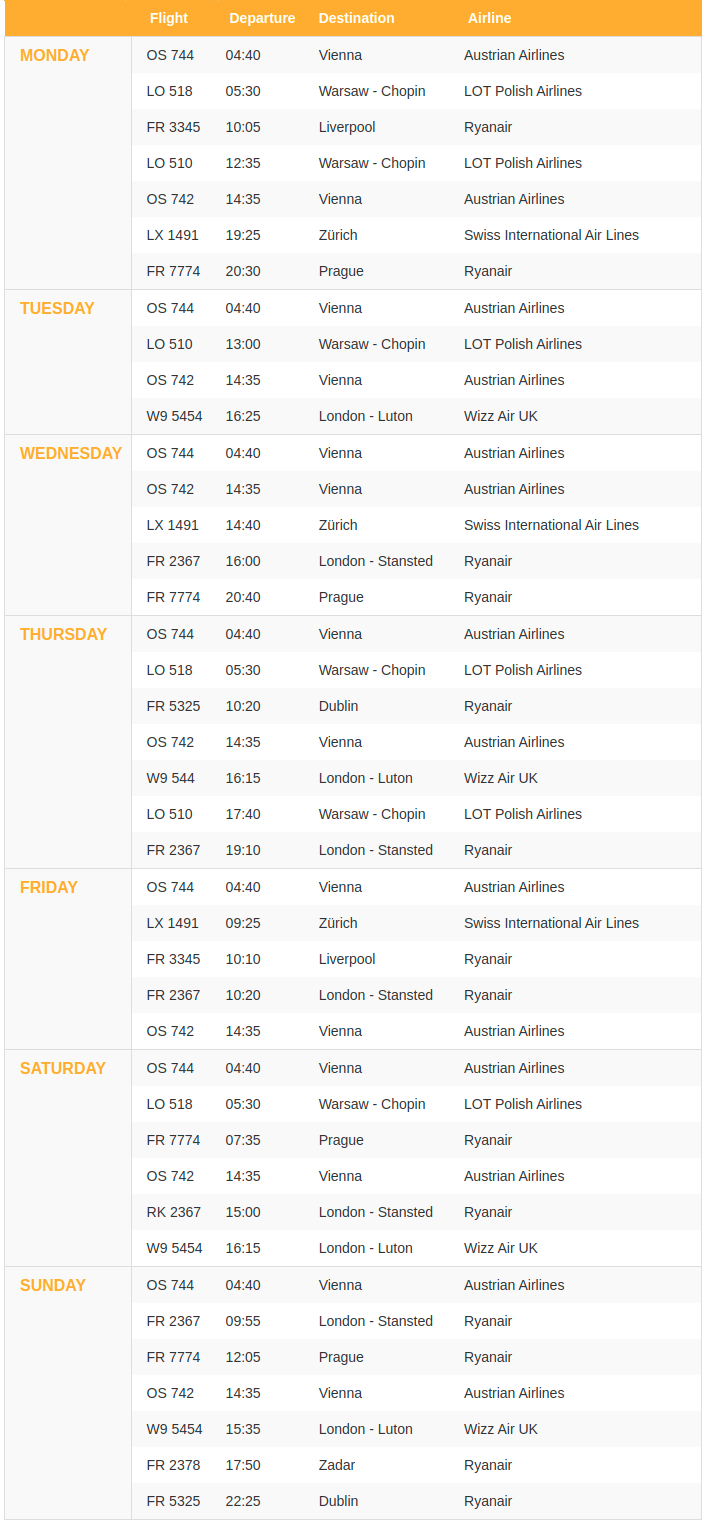
\includegraphics[height=\textheight]{kosice/airport/flights}
		}

		\only<2>{
		\begin{columns}
			\begin{column}{.5\textwidth}
				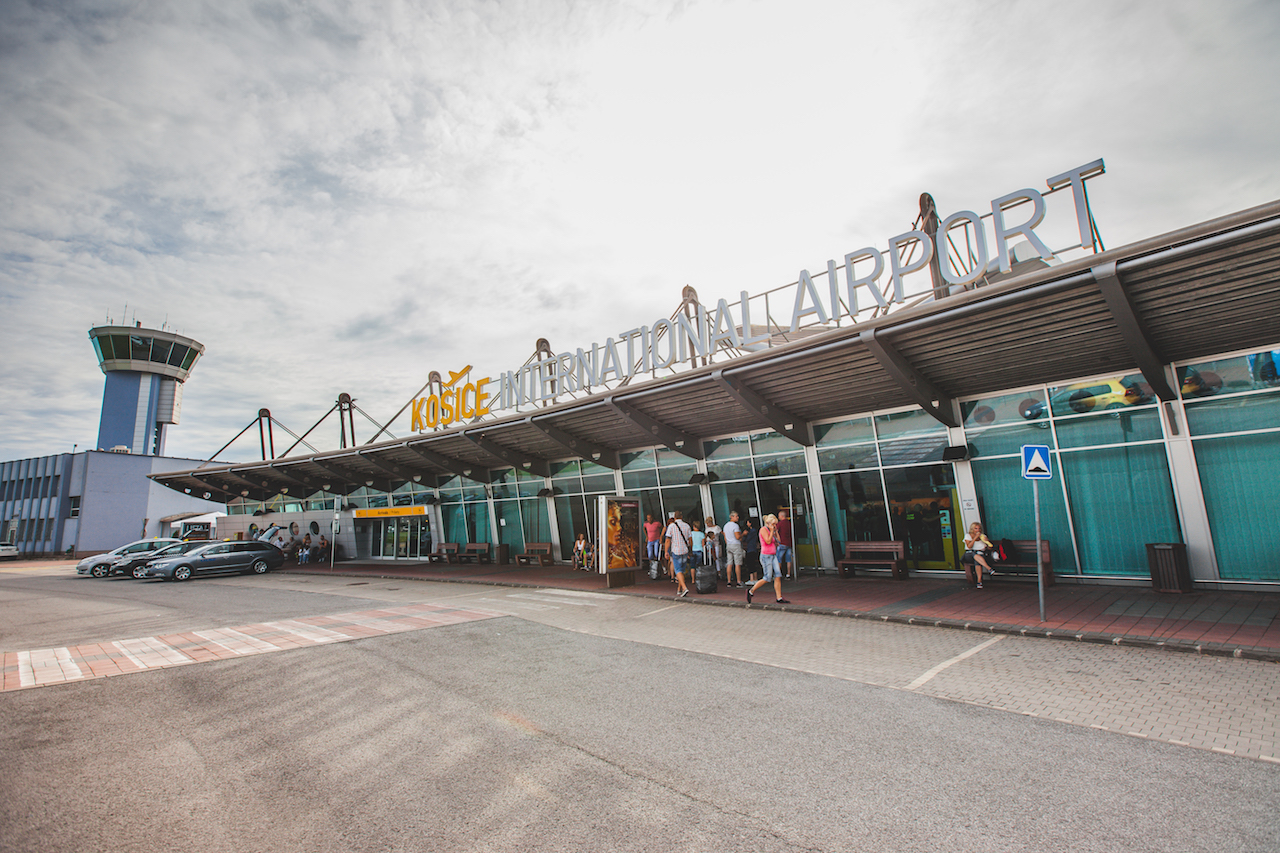
\includegraphics[width=\textwidth]{kosice/airport/1}
			\end{column}
			\begin{column}{.5\textwidth}
				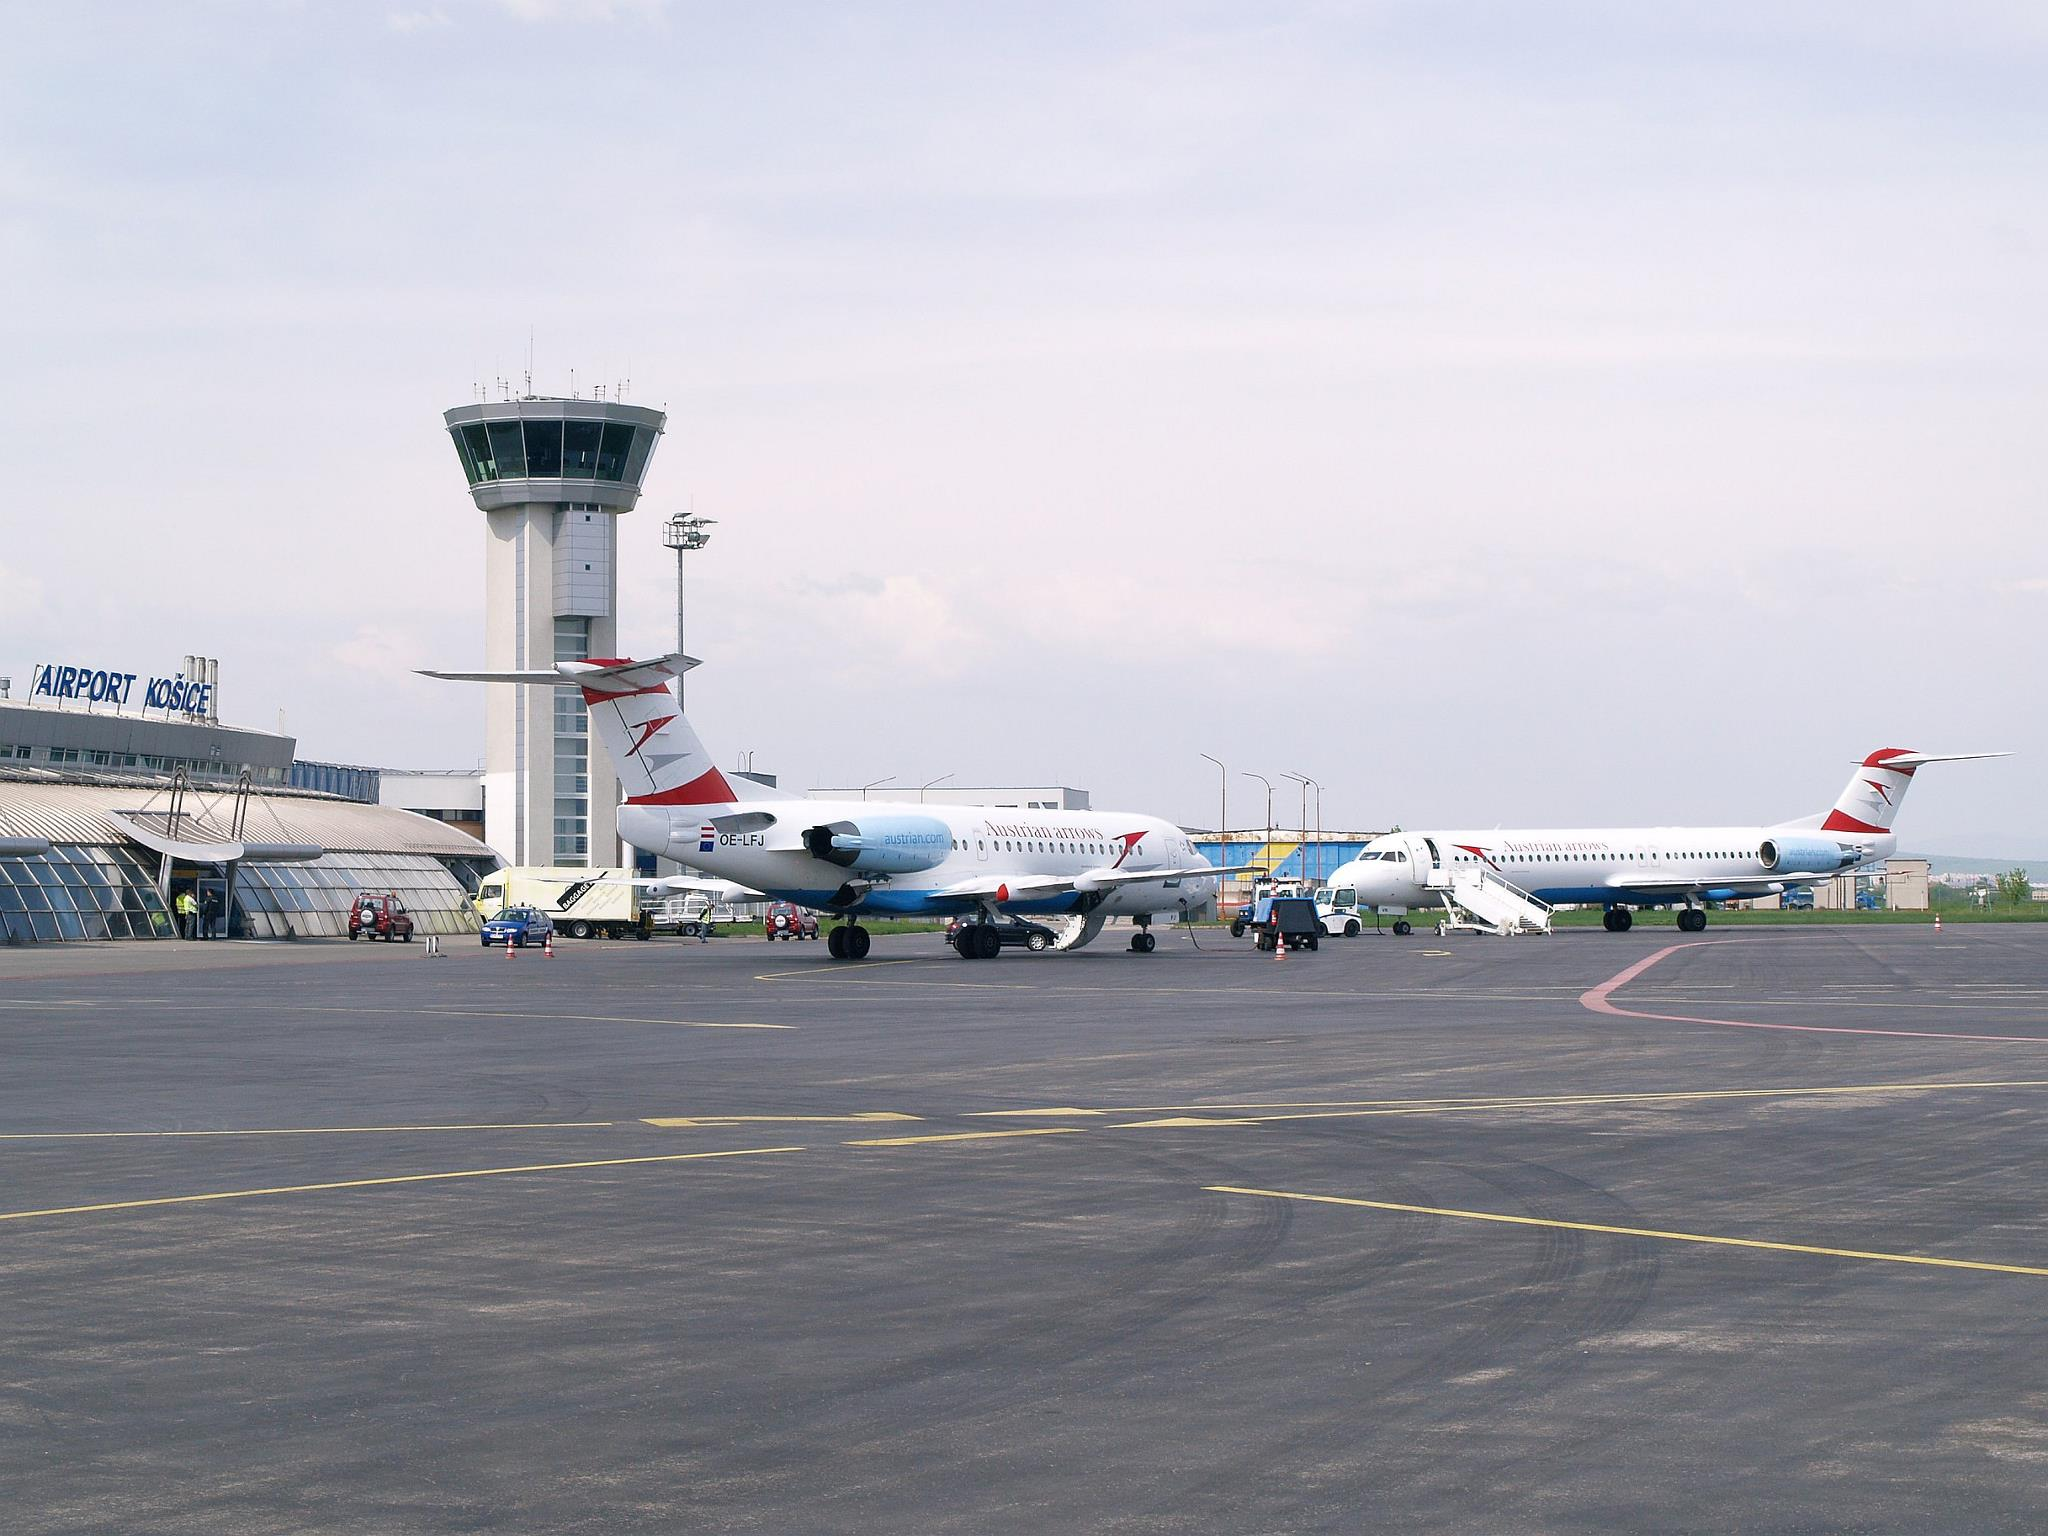
\includegraphics[width=\textwidth]{kosice/airport/2}
			\end{column}
		\end{columns}
		}
		
		\pause
		
		\begin{itemize}
			\item Flights from all around the world
		\end{itemize}
	\end{frame}

	\begin{frame}
		\frametitle{DPMK: Dopravný podnik mesta Košice, a.s.}
		
		\only<1>{
		\begin{columns}
			\begin{column}{.5\textwidth}
				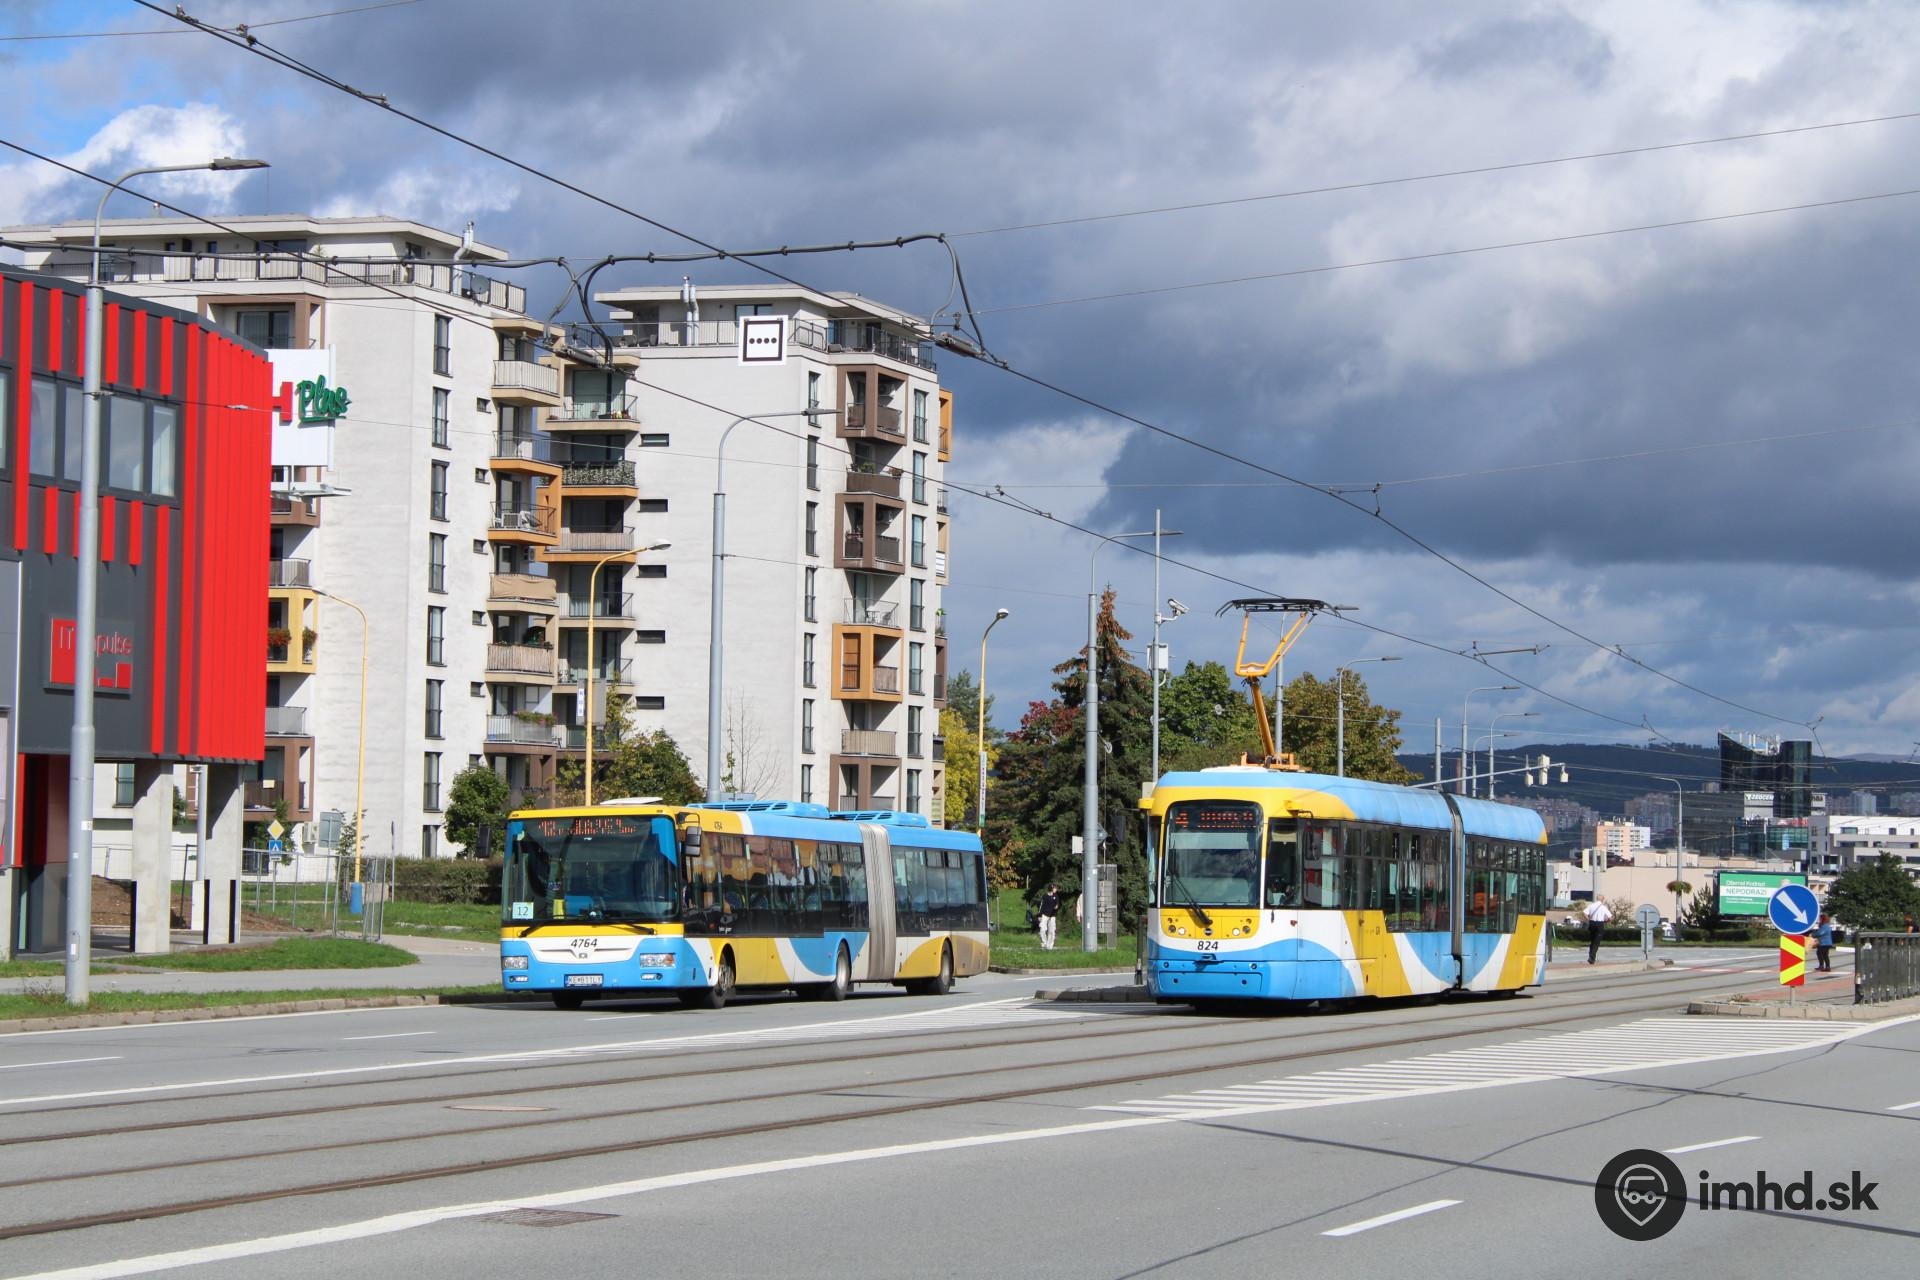
\includegraphics[width=\textwidth]{kosice/mhd}
			\end{column}
			\begin{column}{.5\textwidth}
				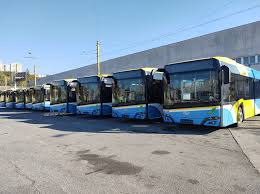
\includegraphics[width=\textwidth]{kosice/mhd2}
			\end{column}
		\end{columns}
		}

		\only<2>{
		\begin{columns}
			\begin{column}{.22\textwidth}
				\centering
				\Large \textbf{1.}\\[1em]
				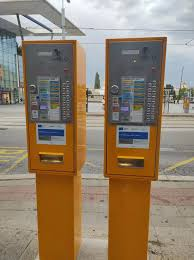
\includegraphics[width=\textwidth]{kosice/automat}
			\end{column}
			\begin{column}{.37\textwidth}
				\centering
				\Large \textbf{2.}\\[1em]
				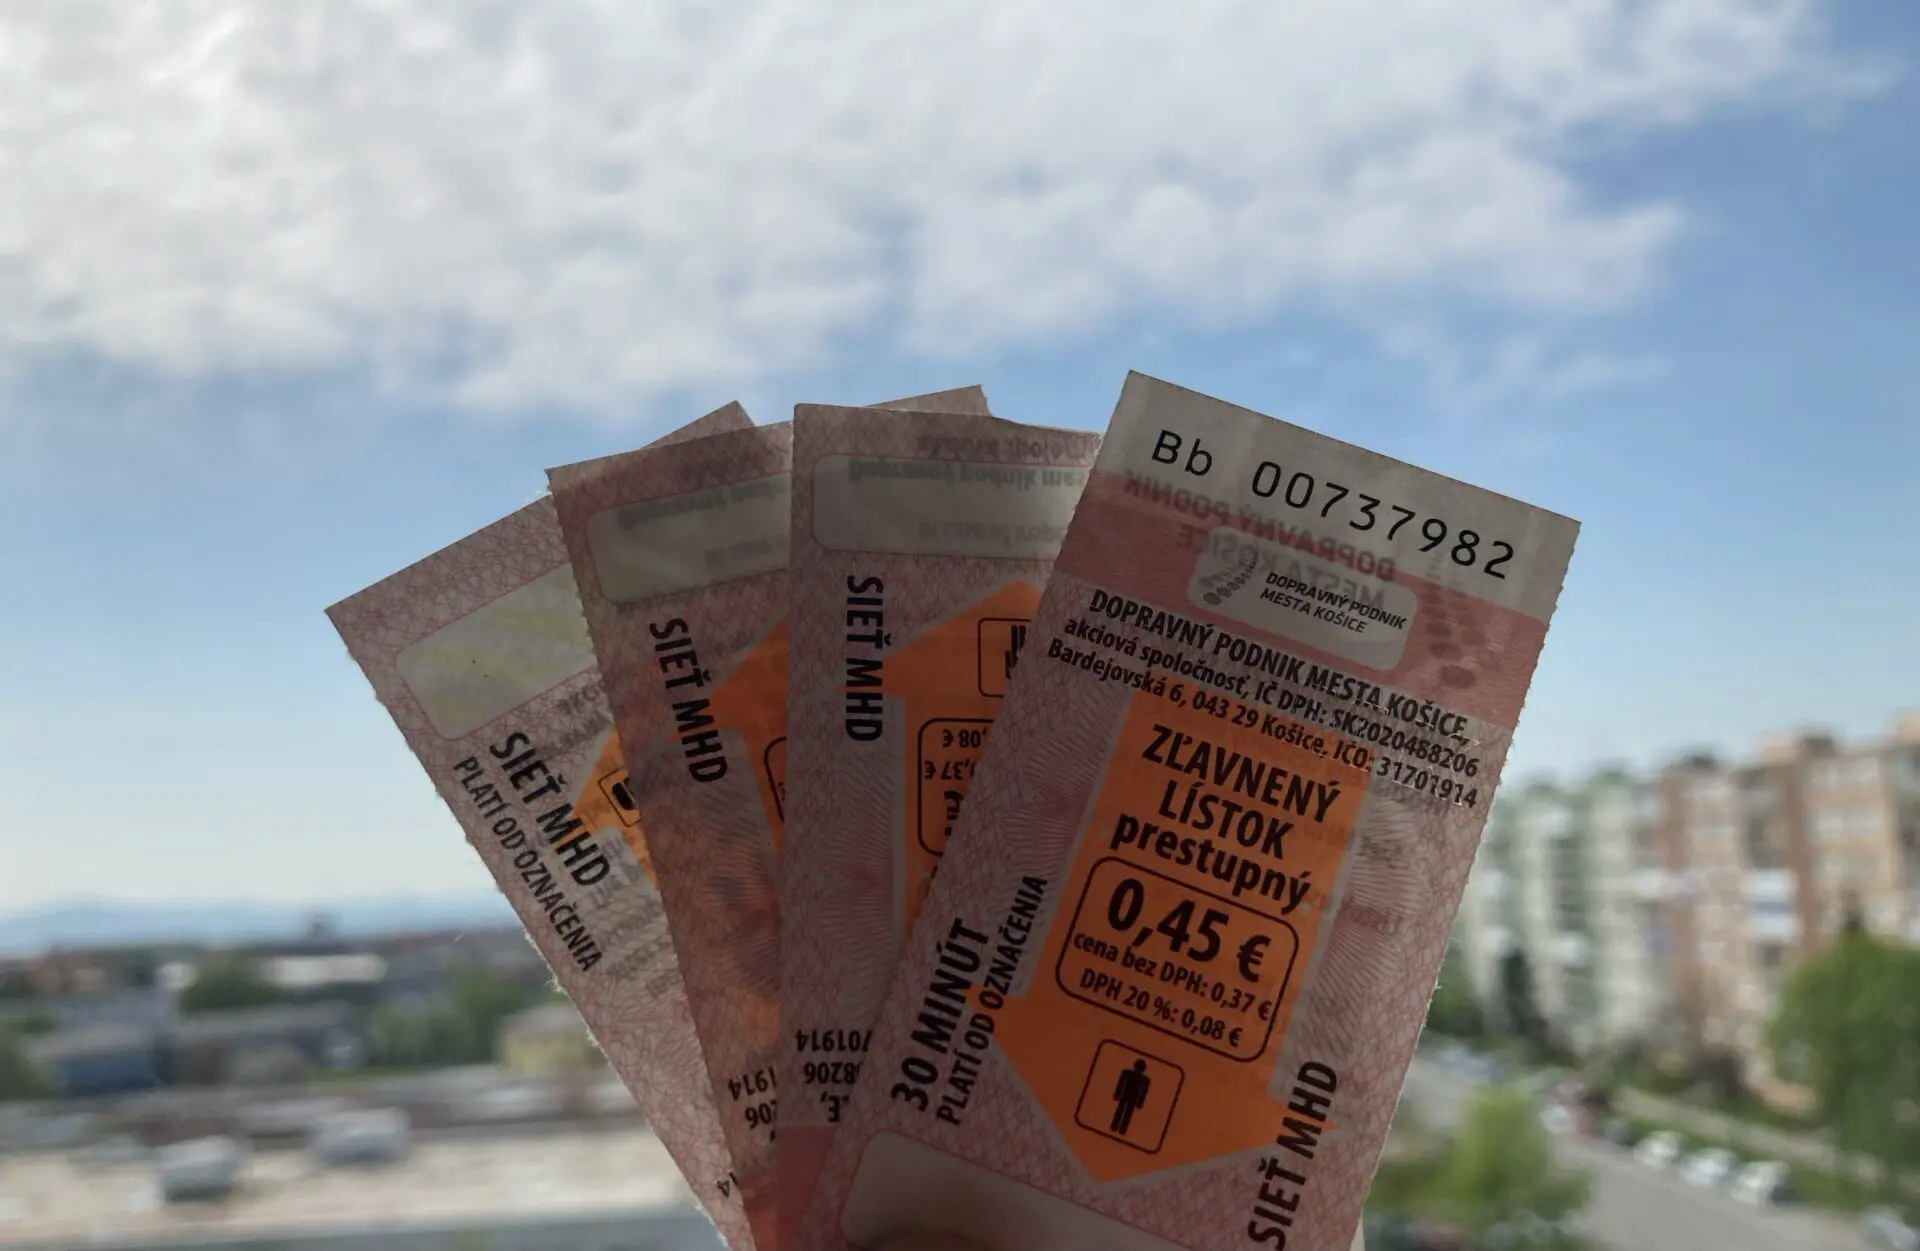
\includegraphics[width=\textwidth]{kosice/listok}
			\end{column}
			\begin{column}{.37\textwidth}
				\centering
				\Large \textbf{3.}\\[1em]
				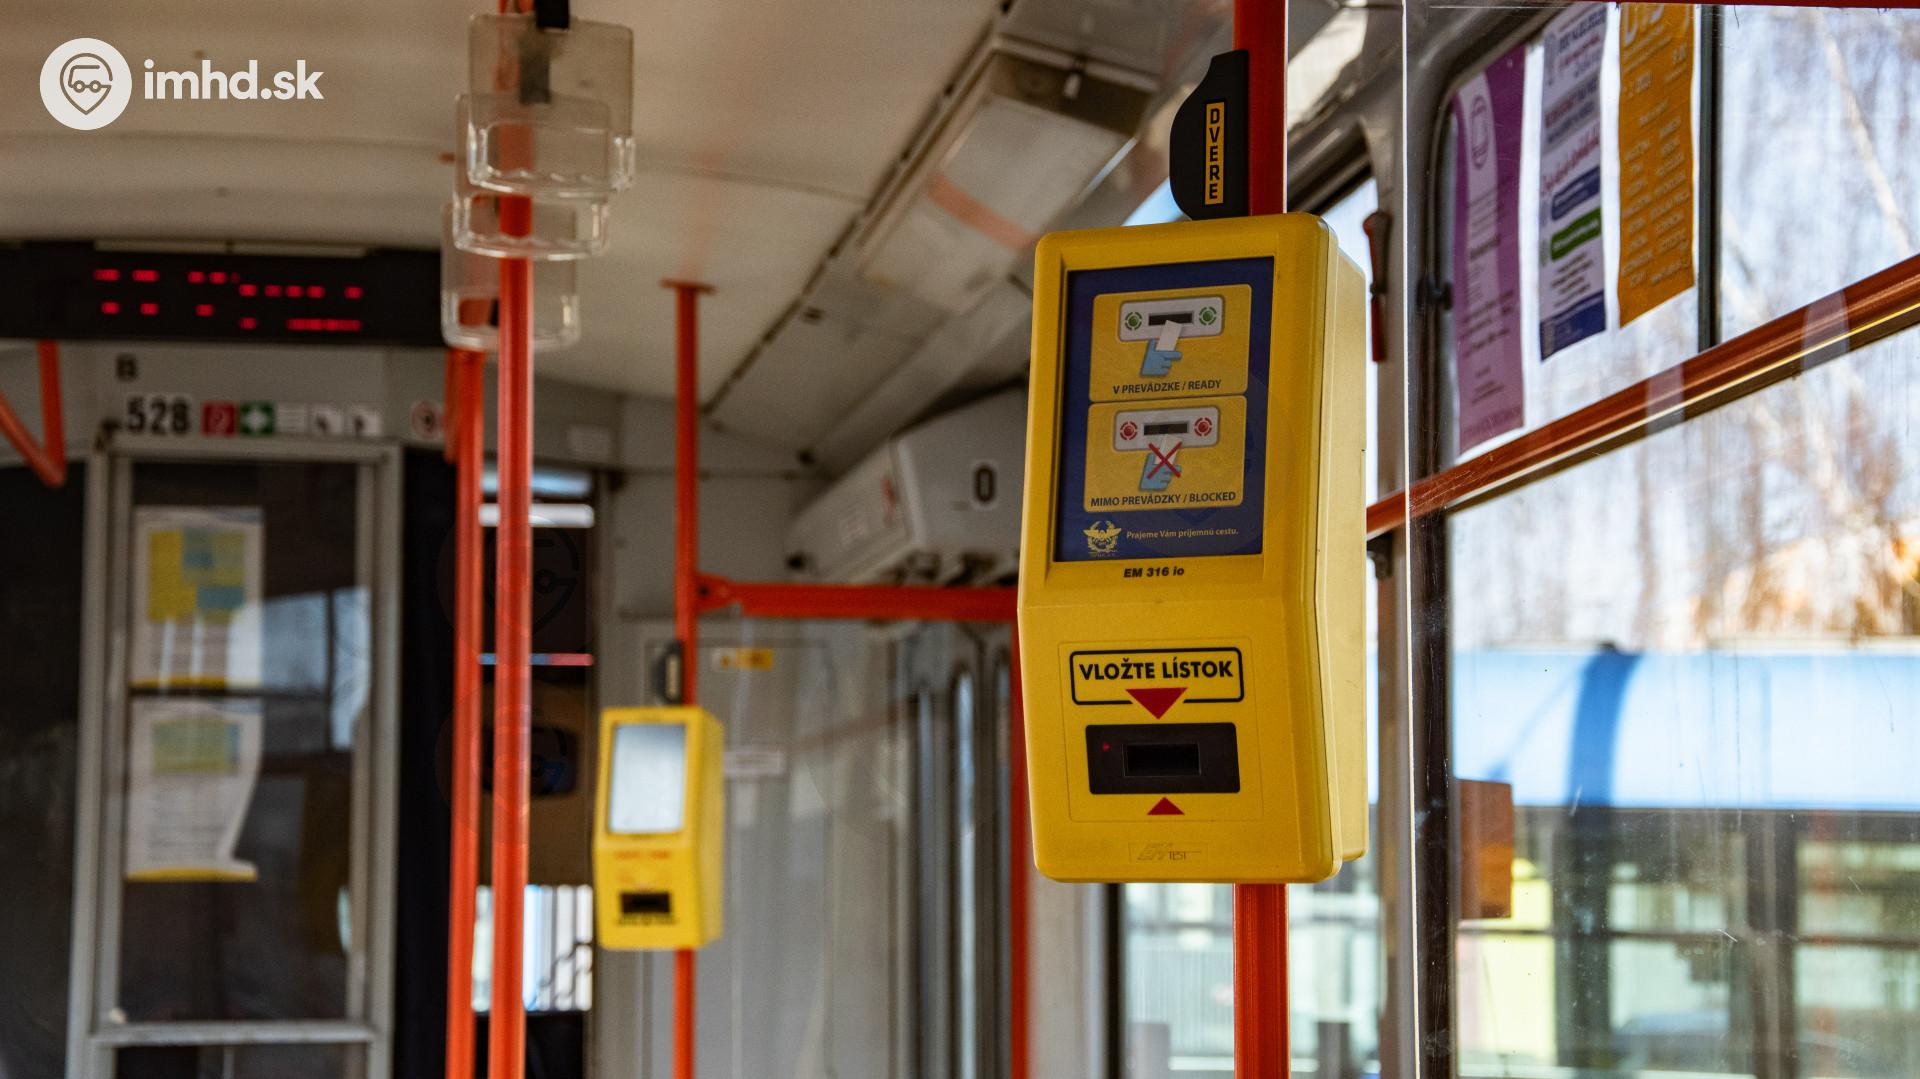
\includegraphics[width=\textwidth]{kosice/ticket-stamper}
			\end{column}
		\end{columns}
		}
	\end{frame}

	\begin{frame}
		\frametitle{Things to see}

		\centering		

		\only<1>{
		\Large Dom sv. Alžbety\\[0.5em]
		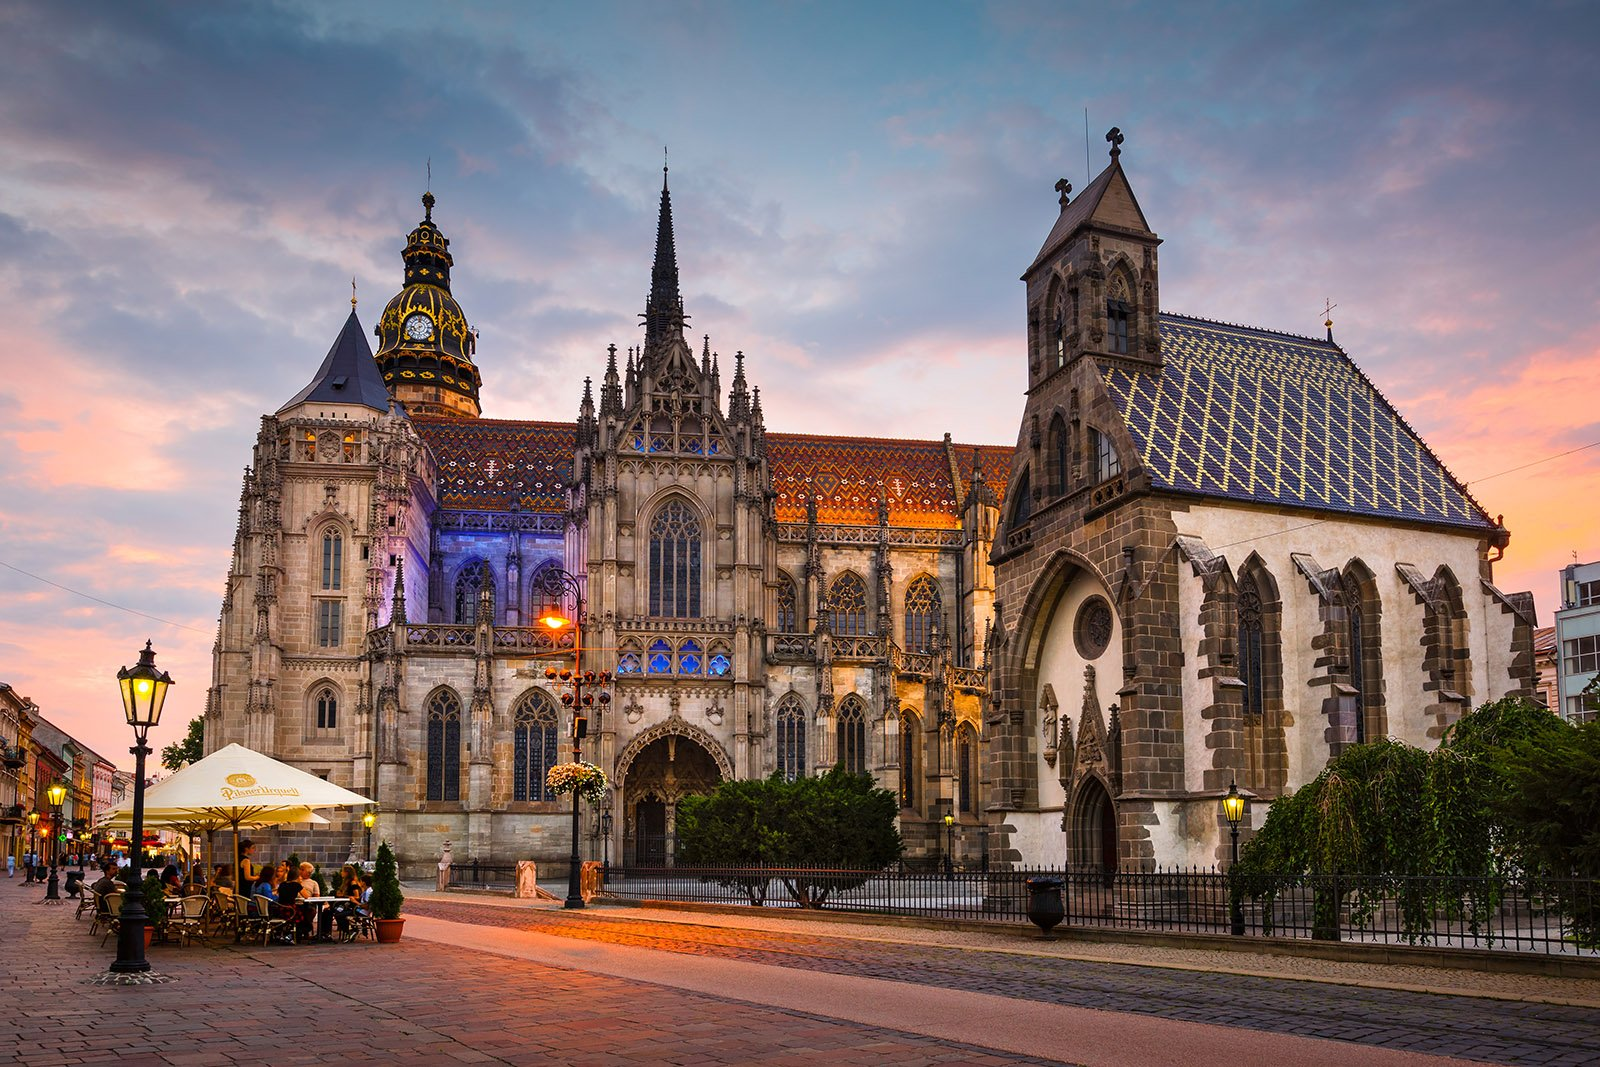
\includegraphics[width=\textwidth]{kosice/centrum}
		}
		\only<2>{
		\Large National Theatre Košice\\[0.5em]
		\includegraphics[width=\textwidth]{kosice/divadlo}
		}
		\only<3>{
		\Large National Theatre Košice\\[0.5em]
		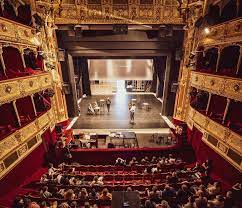
\includegraphics[width=\textwidth]{kosice/divadlo_vnutry}
		}
	\end{frame}

	\begin{frame}
		\frametitle{Accomodation}

		\only<1>{
		\begin{columns}
			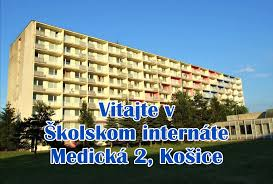
\includegraphics[width=\textwidth]{kosice/internat}
		\end{columns}
		}
		\only<2>{
		\begin{columns}
			\begin{column}{.5\textwidth}
				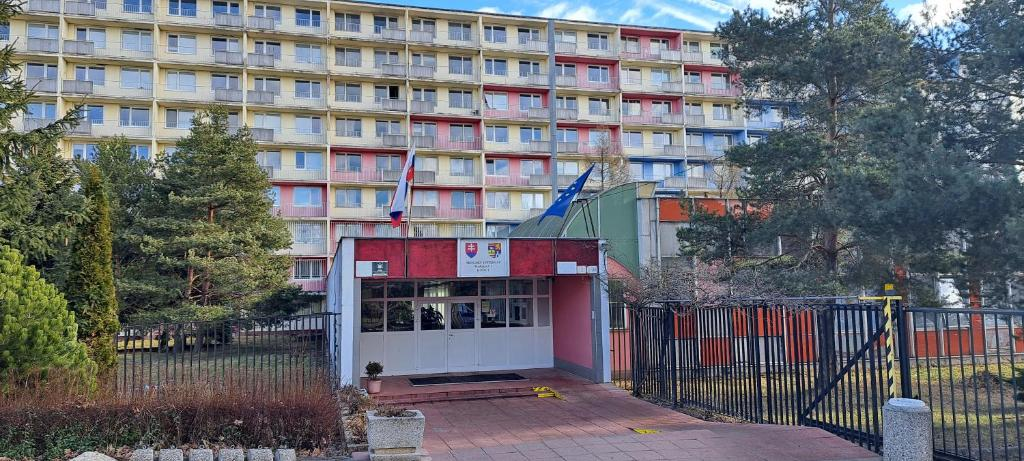
\includegraphics[width=\textwidth]{kosice/internat1}
			\end{column}
			\begin{column}{.5\textwidth}
				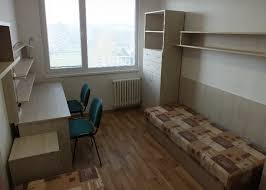
\includegraphics[width=\textwidth]{kosice/internat_vnutry}
			\end{column}
		\end{columns}
		}

	\end{frame}

	\section{Day 1. cost summarization}

	\begin{frame}
		\frametitle{Day 1. cost summarization}

		\begin{itemize}
			\item 24h ticket 3.5€
			\item Giuseppe Verdo: NABUCCO 7.8€
			\item Accomodation 10€
		\end{itemize}

		Total cost: 21.3€
	\end{frame}

	\section{Day 2.}

	\begin{frame}
		\frametitle{Transport}

		\begin{itemize}
			\item Buses
			\pause
			\item Trains
		\end{itemize}

		\pause

		\begin{columns}
		\begin{column}{.5\textwidth}
		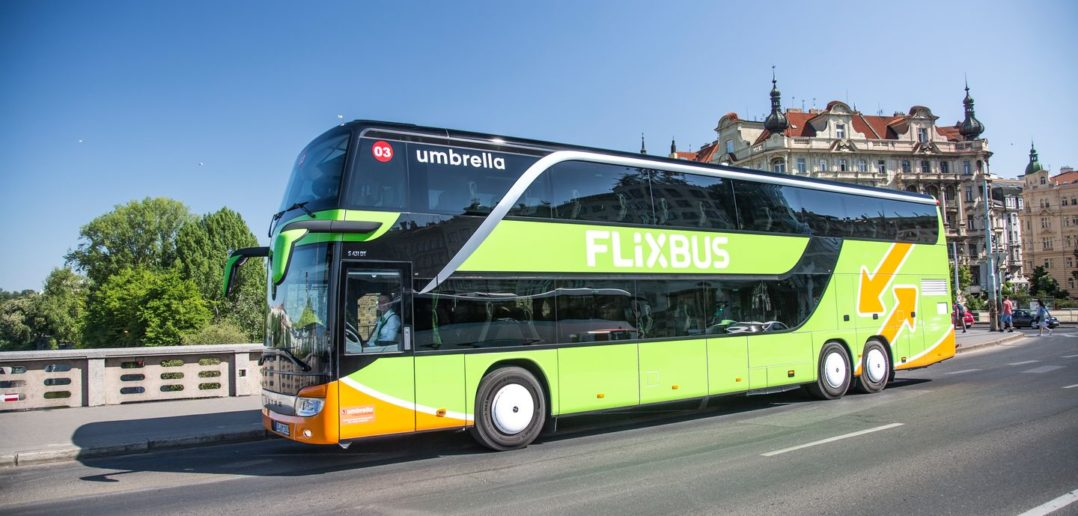
\includegraphics[width=\textwidth]{flixbux}
		\end{column}
		
		\begin{column}{.5\textwidth}
		So called "Čachtická strela" (no joke)\\[0.5em]
		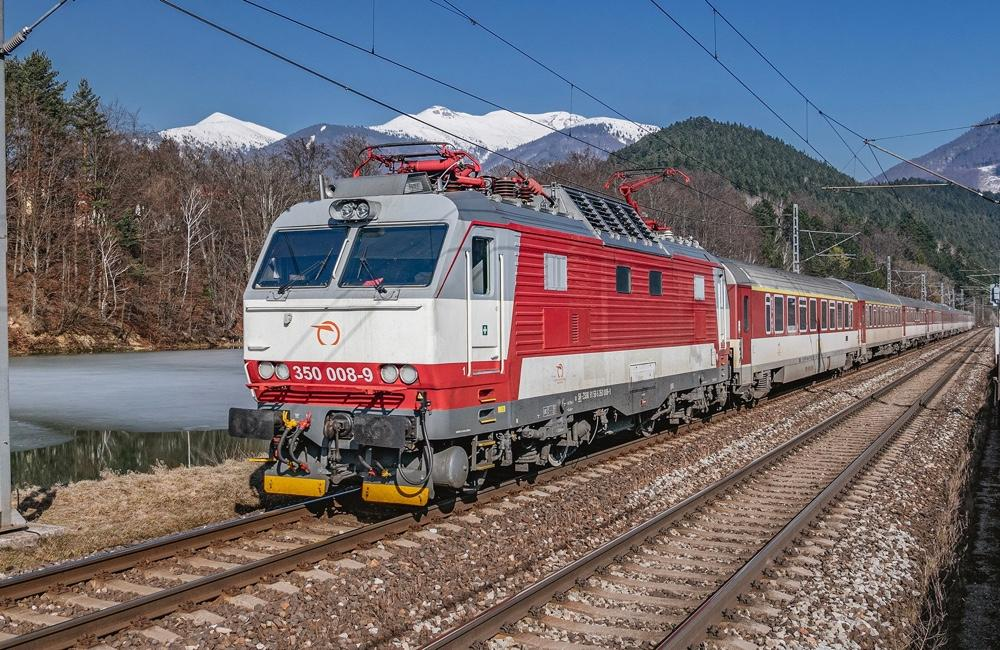
\includegraphics[width=\textwidth]{vlak}
		\end{column}
		\end{columns}
	\end{frame}

	\begin{frame}
		\frametitle{Spišský hrad}

		\note{Slovakia is a country of castles, most castles per capita in europe}
		\begin{columns}
			\begin{column}{.5\textwidth}
				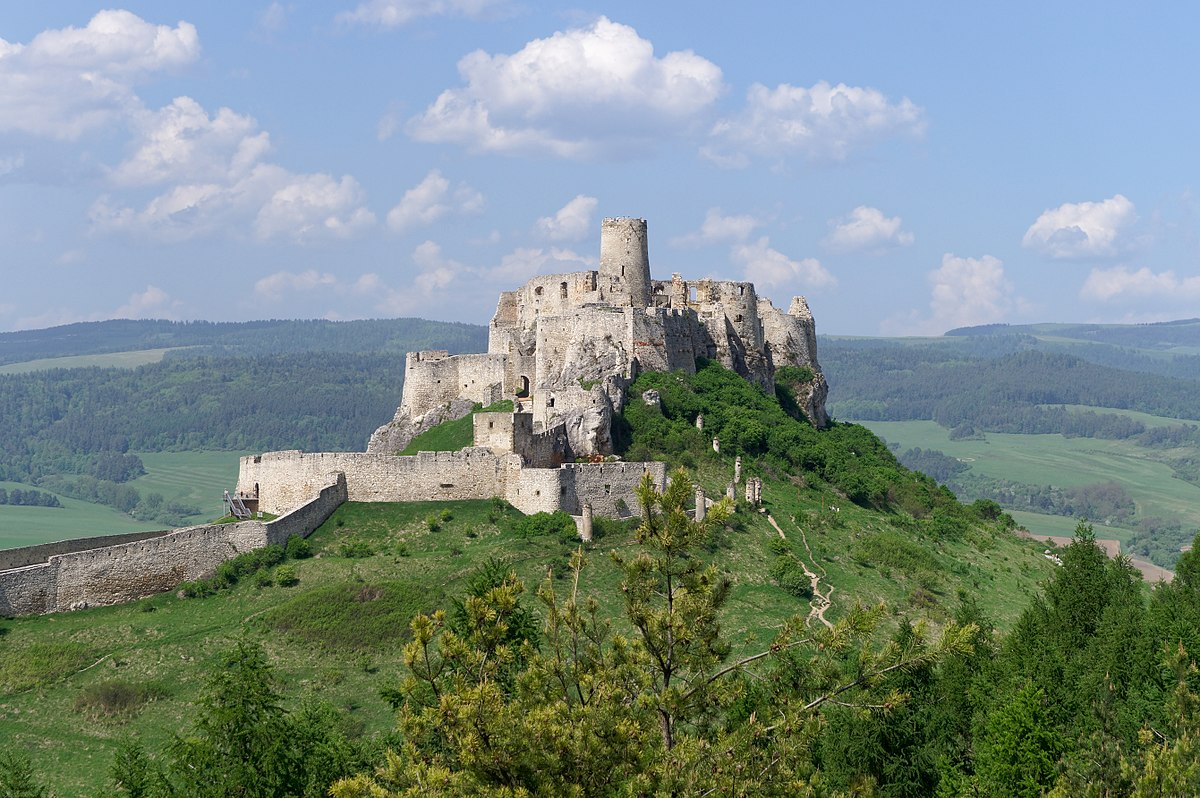
\includegraphics[width=\textwidth]{day2/hrad}
			\end{column}
			\begin{column}{.5\textwidth}
				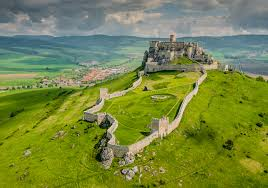
\includegraphics[width=\textwidth]{day2/hrad-topdown}
			\end{column}
		\end{columns}

		\pause

		\vspace{1em}
		\begin{itemize}
			\item One of the biggest castles in central europe
			\item 4 hectares area
		\end{itemize}
	\end{frame}


	\begin{frame}
		\note{First Imagine you could go to a place with endless moutains and nature, now imagine it's in slovakia}
		\only<2>{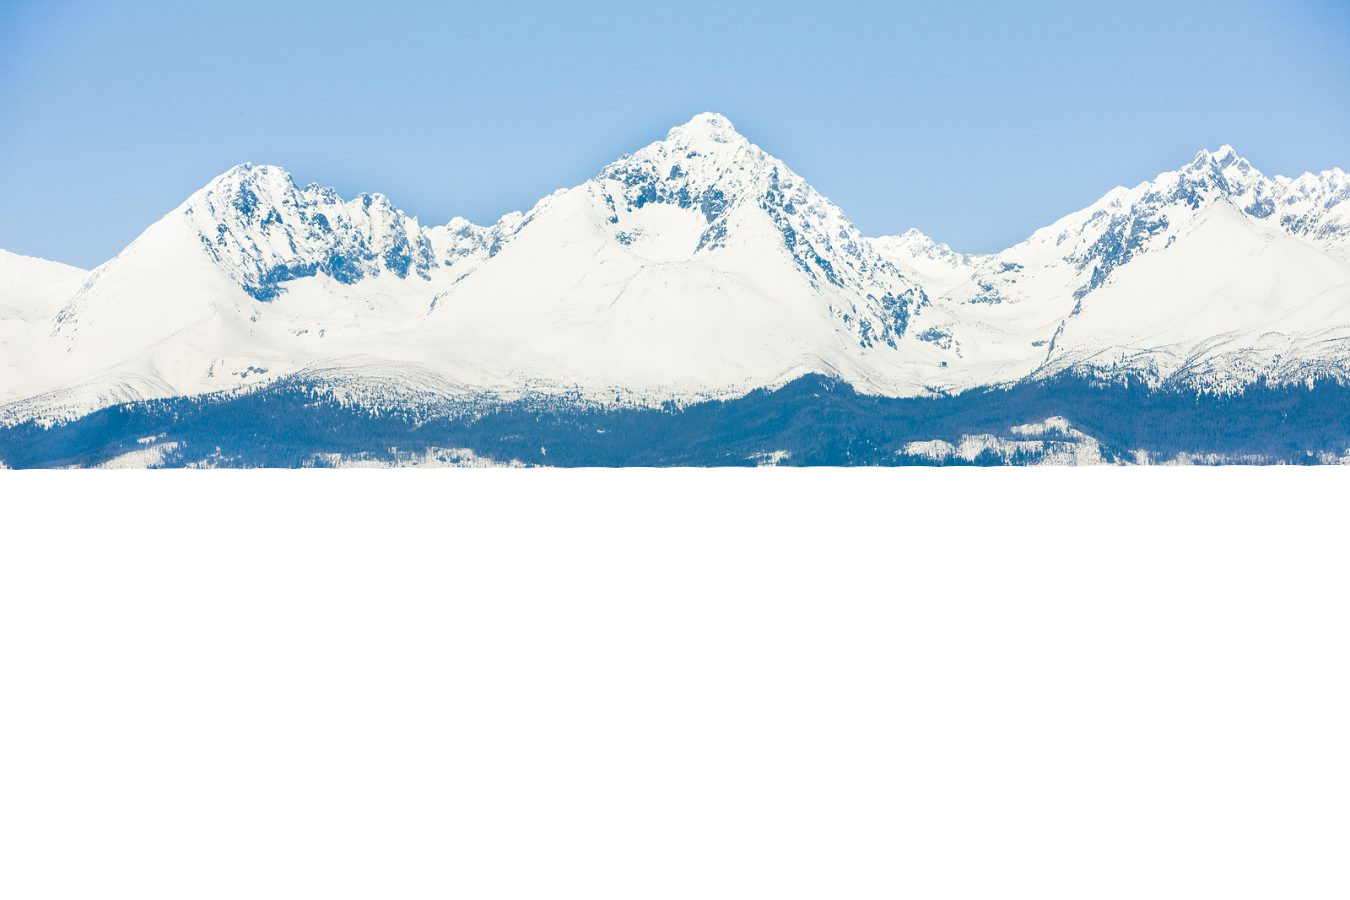
\includegraphics[width=\textwidth]{day2/poprad-polovica}}
		\only<3->{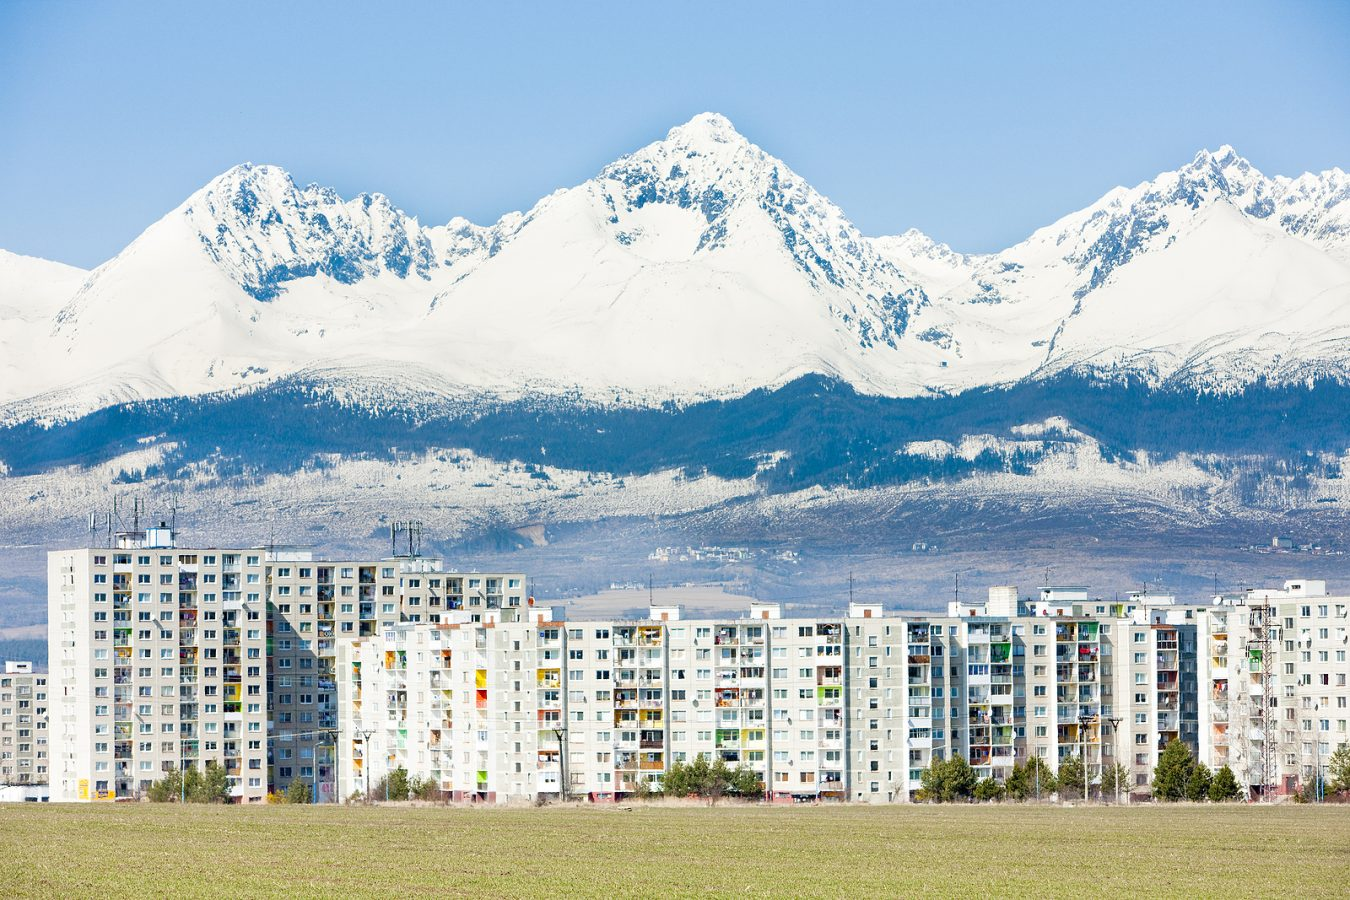
\includegraphics[width=\textwidth]{day2/poprad}}

		\only<4>{
			\frametitle{Poprad}
			\begin{itemize}
				\item Provides great access to High Tatras
			\end{itemize}
		}
	\end{frame}

	\begin{frame}
		\frametitle{Poprad}

		\begin{columns}
			\frametitle{VÝHĽAD Tatry - ISC RESORT MLYNICA}
			\begin{column}{0.5\textwidth}
				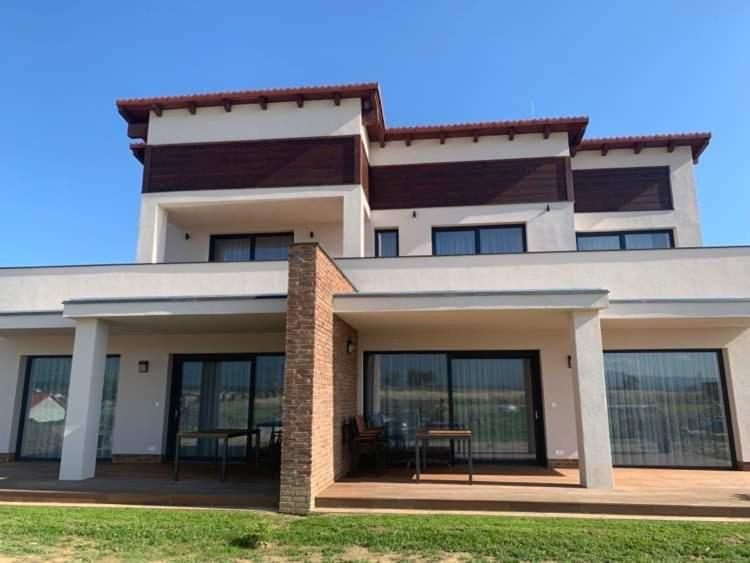
\includegraphics[width=\textwidth]{day2/hotel}
			\end{column}
			\begin{column}{0.5\textwidth}
				\begin{itemize}
					\item Apparently just a house
				\end{itemize}
			\end{column}
		\end{columns}
	\end{frame}

	\section{Day 2. cost summarization}

	\begin{frame}
		\frametitle{Day 2. cost summarization}

		\begin{itemize}
			\item Špišský hrad ticket 8€
			\item ISC RESORT MLYNICA 50€
		\end{itemize}
	\end{frame}

	\section{Day 3.}

	\begin{frame}
		\frametitle{All aboard the winter express}
		
		\only<1>{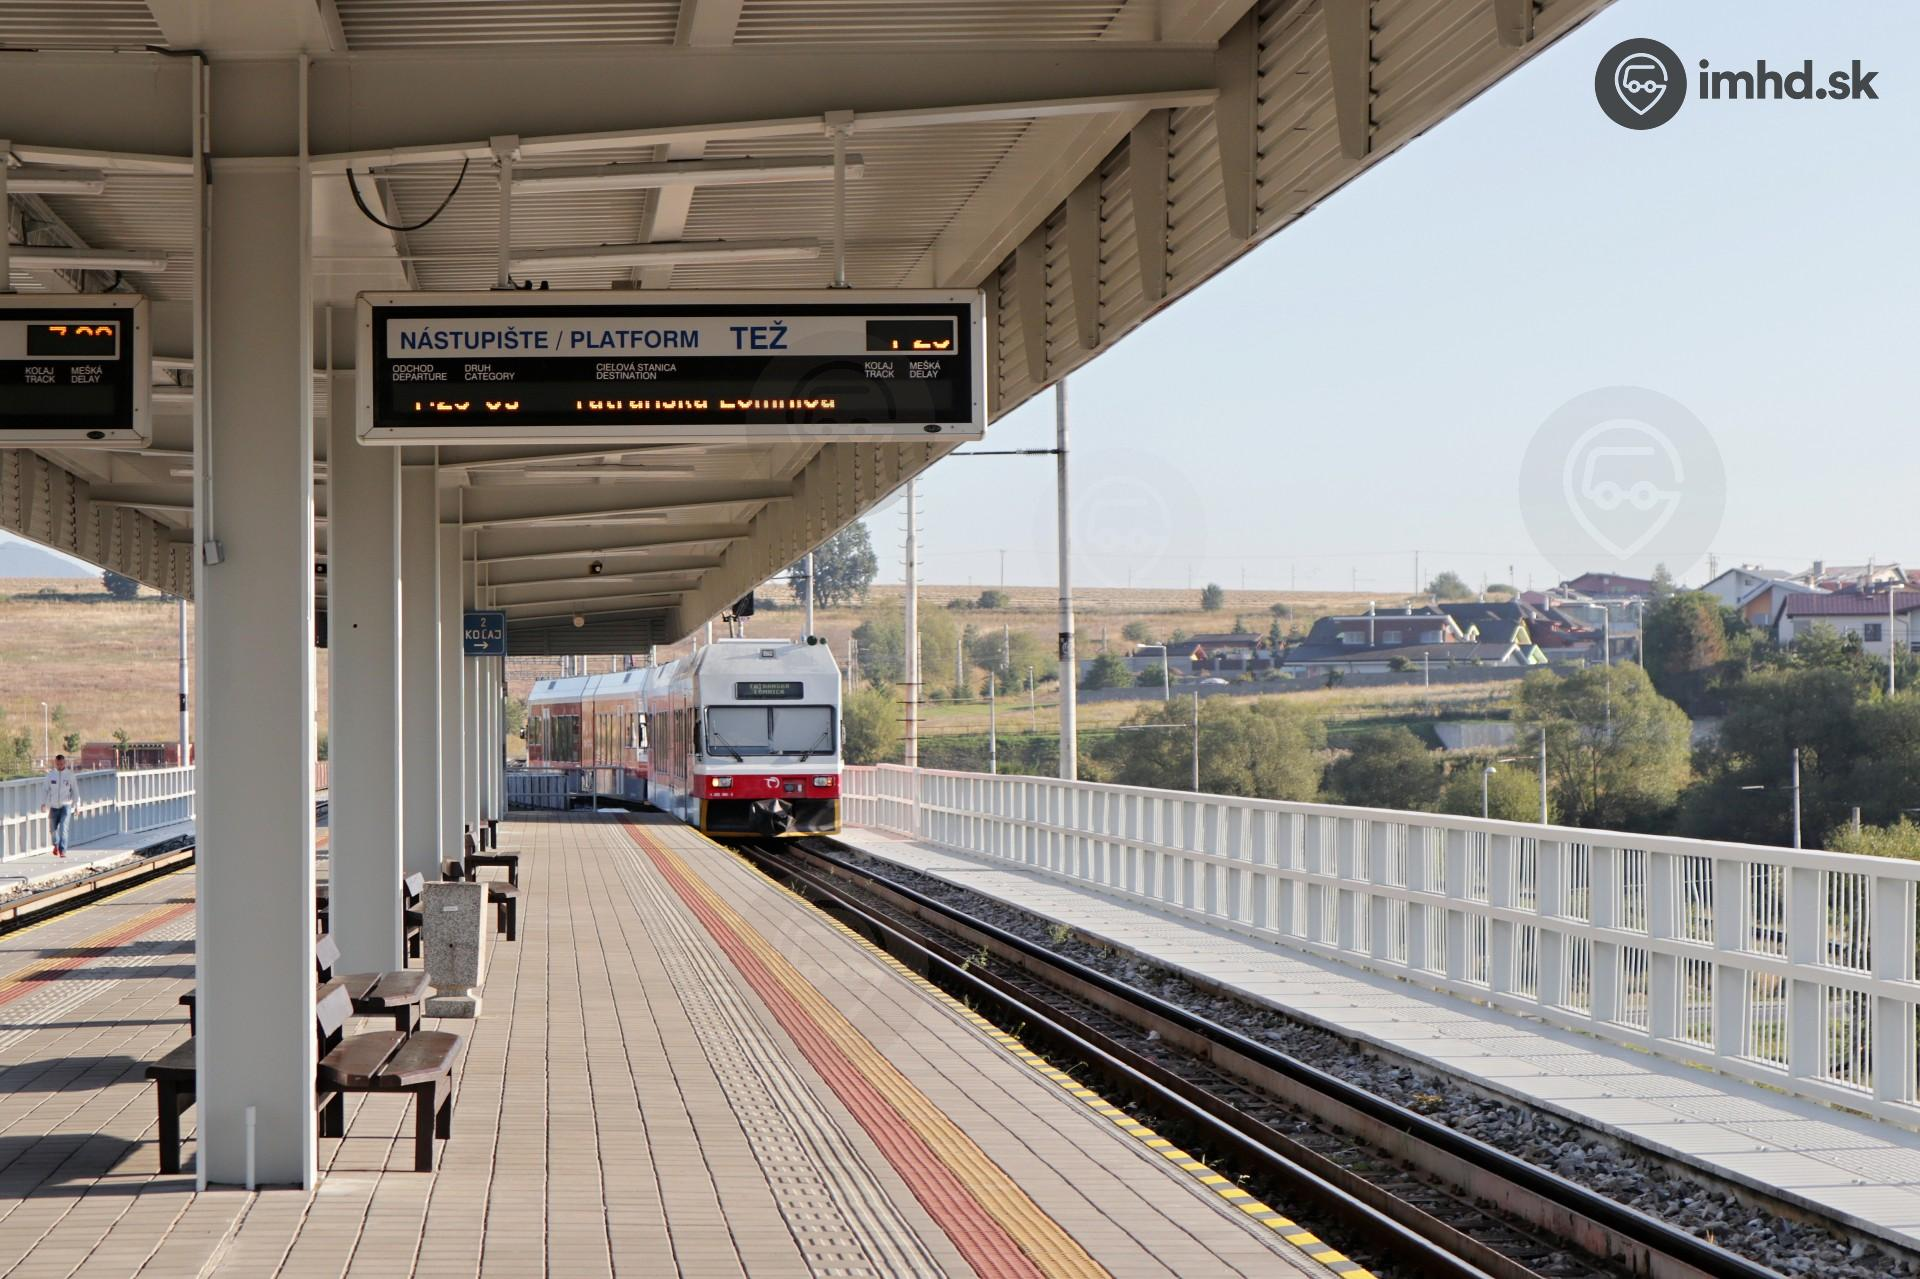
\includegraphics[width=\textwidth]{day3/stanica}}
		\only<2>{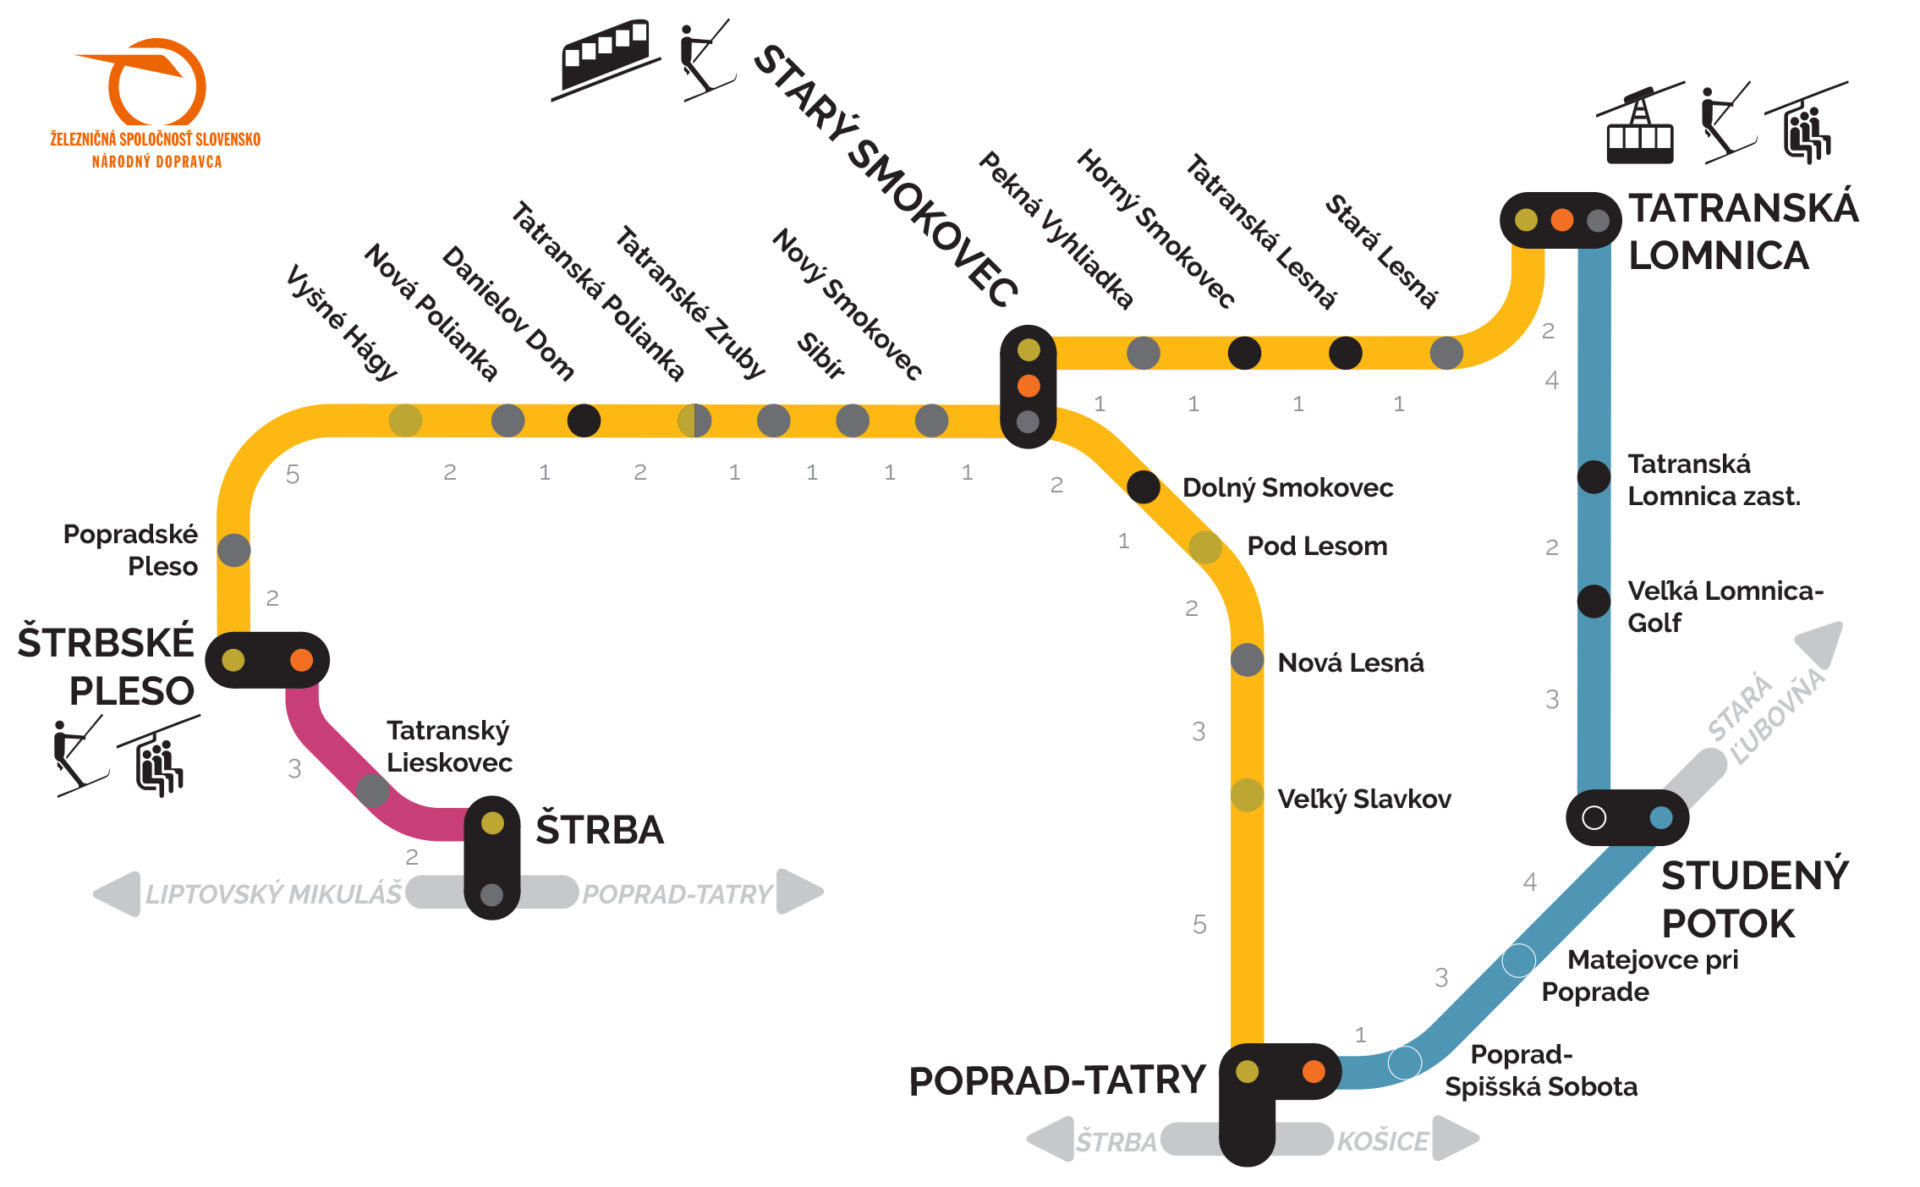
\includegraphics[width=\textwidth]{day3/mapa}}
		\only<3>{
			\begin{columns}
				\begin{column}{0.5\textwidth}
				Štrbské pleso
				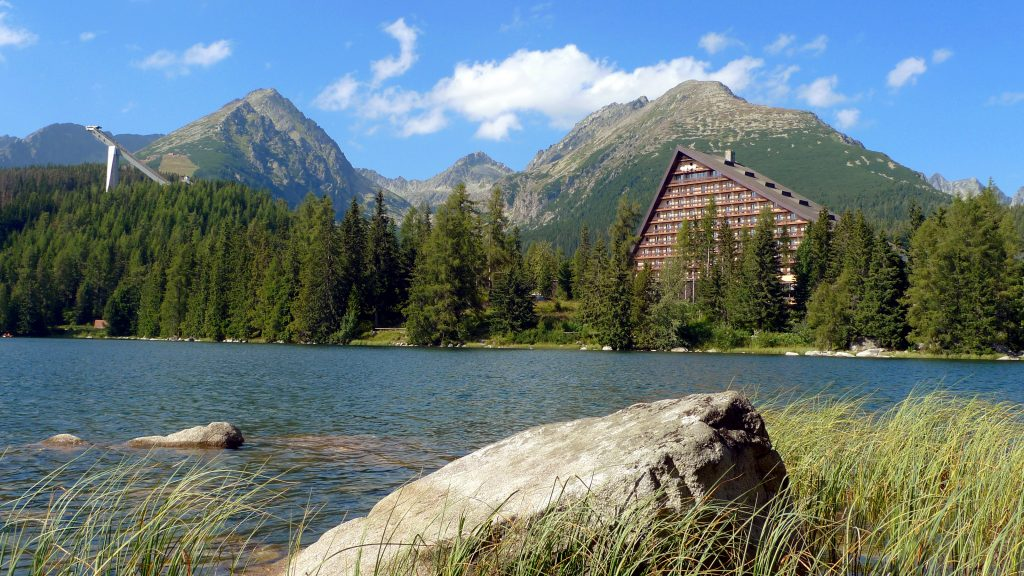
\includegraphics[width=\textwidth]{day3/pleso1}
				\end{column}
				\begin{column}{0.5\textwidth}
				Popradské pleso
				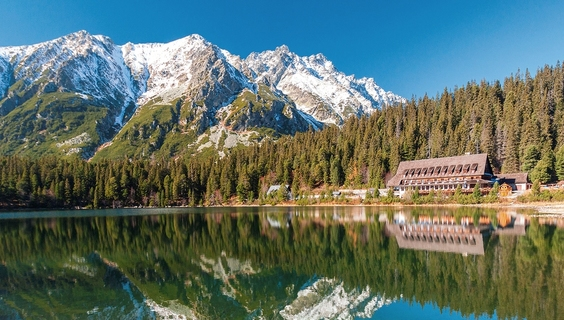
\includegraphics[width=\textwidth]{day3/pleso2}
				\end{column}
			\end{columns}
		}
		\only<4>{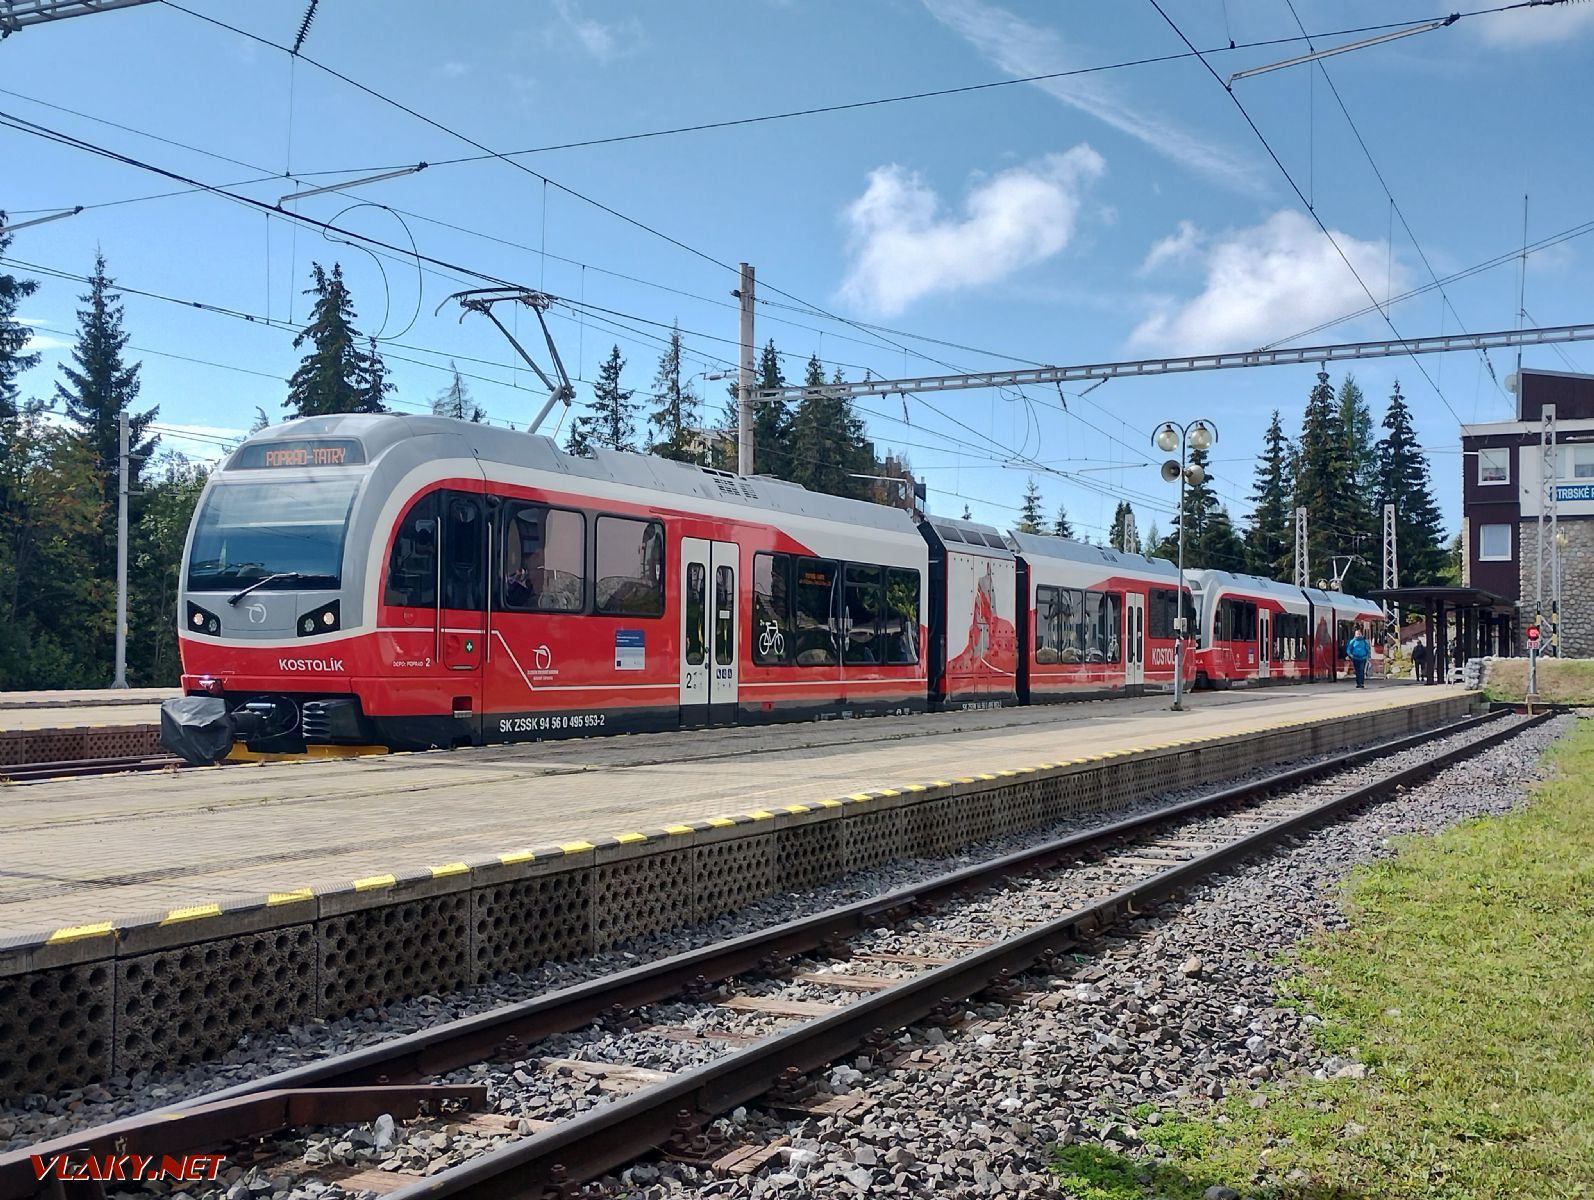
\includegraphics[width=\textwidth]{day3/zubacka}}
		\only<5>{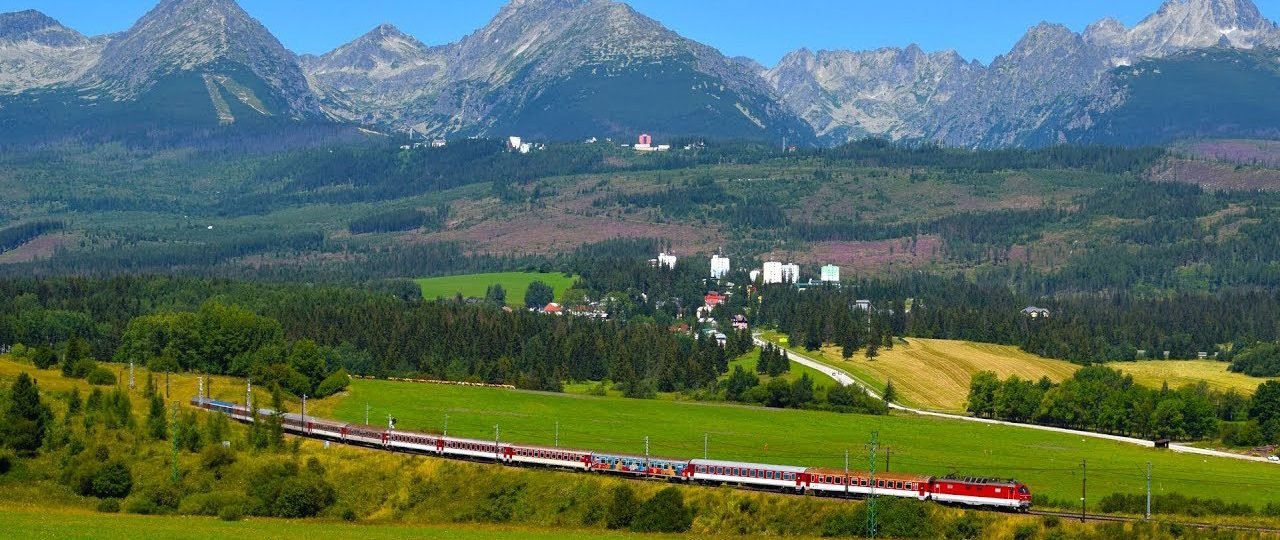
\includegraphics[width=\textwidth]{day3/back}}
	\end{frame}
	
	\section{Day 3. cost summarization}
	\begin{frame}
		\frametitle{Day 3. cost summarization}

		\begin{itemize}
			\item Train tickets 3 * 2.5€
			\item ISC RESORT MLYNICA 50€
		\end{itemize}
	\end{frame}

	\section{Day 4.}

	\begin{frame}
		\frametitle{Liptovská Mara}

		\begin{columns}	
		\begin{column}{0.5\textwidth}
		\centering
		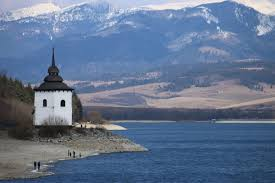
\includegraphics[width=0.7\textwidth]{day4/mara}
		\end{column}
		\begin{column}{0.5\textwidth}
		\centering
		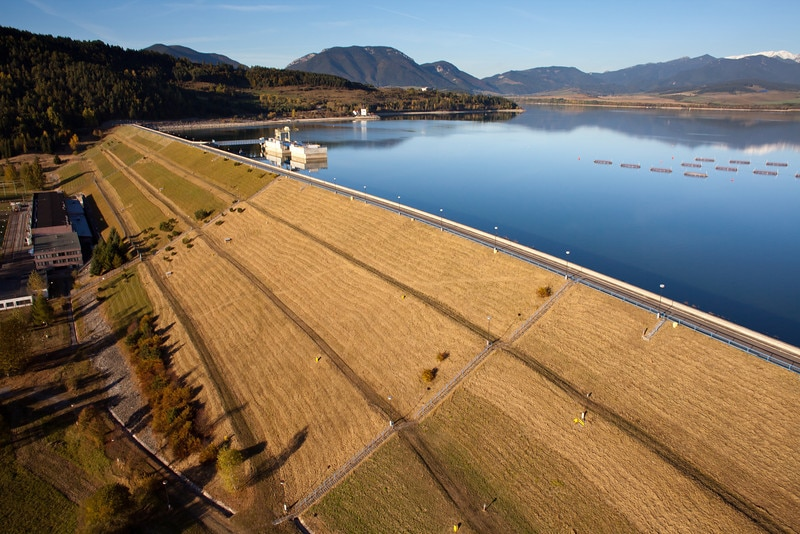
\includegraphics[width=0.7\textwidth]{day4/mara2}
		\end{column}
		\end{columns}
		\vspace{1em}
		\centering
		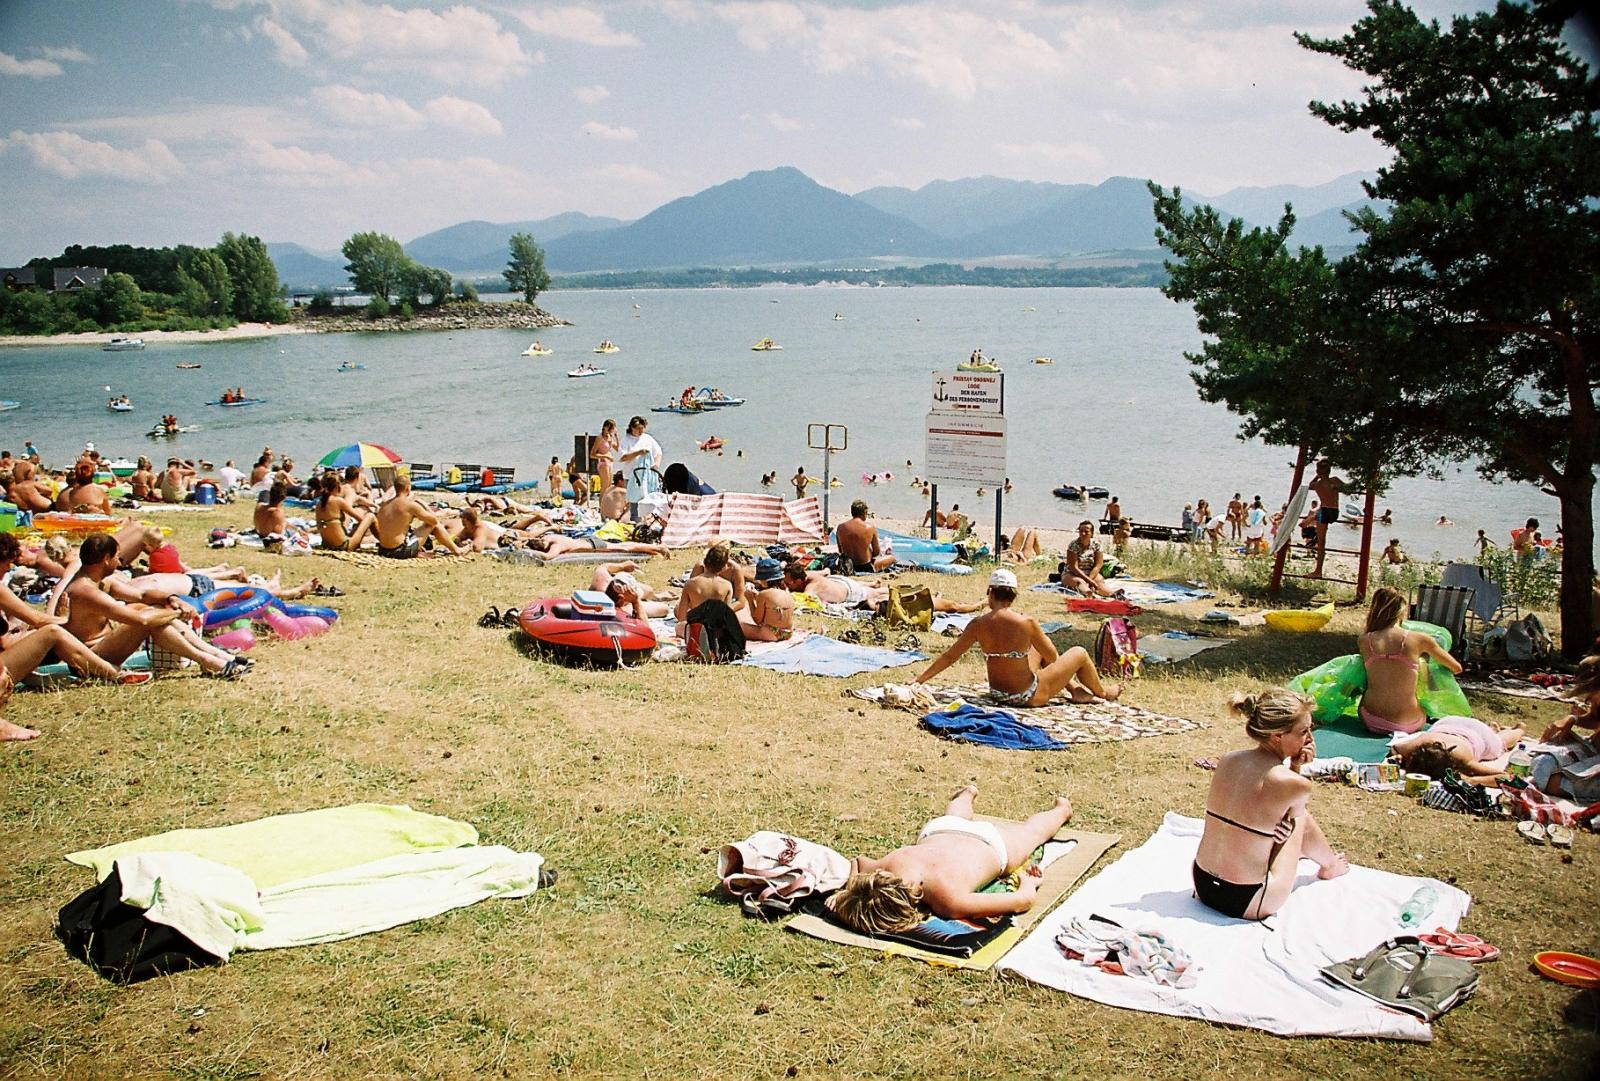
\includegraphics[width=0.5\textwidth]{day4/plaz}
	\end{frame}

	\begin{frame}
		\frametitle{Let's get to the point}
		
		\begin{columns}
		\begin{column}{0.5\textwidth}
		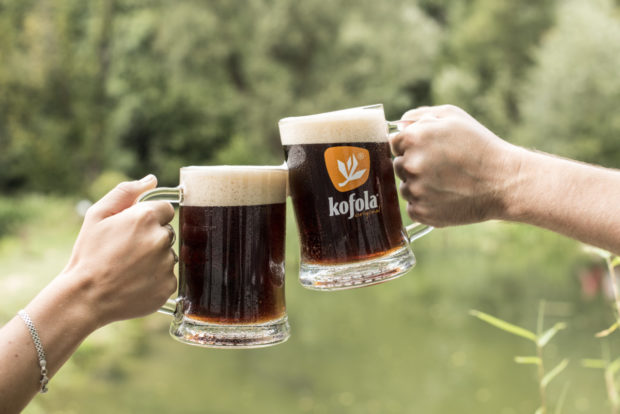
\includegraphics[width=\textwidth]{day4/kofola}
		\end{column}
		\begin{column}{0.5\textwidth}
		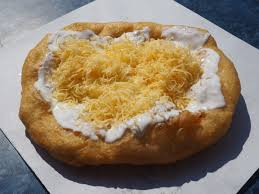
\includegraphics[width=\textwidth]{day4/langos}
		\end{column}
		\end{columns}

		\pause		

		\begin{columns}
		\begin{column}{0.5\textwidth}
		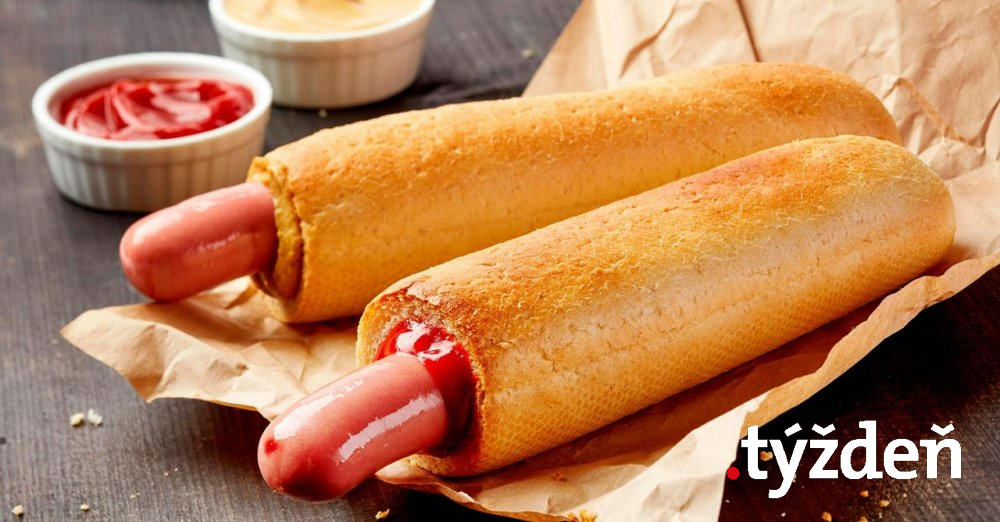
\includegraphics[width=\textwidth]{day4/parok}
		\end{column}
		\begin{column}{0.5\textwidth}
		\centering
		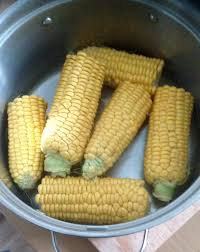
\includegraphics[width=0.6\textwidth]{day4/kukurica}
		\end{column}
		\end{columns}
	\end{frame}

	\begin{frame}
		\frametitle{Liptovský Mikuláš}
		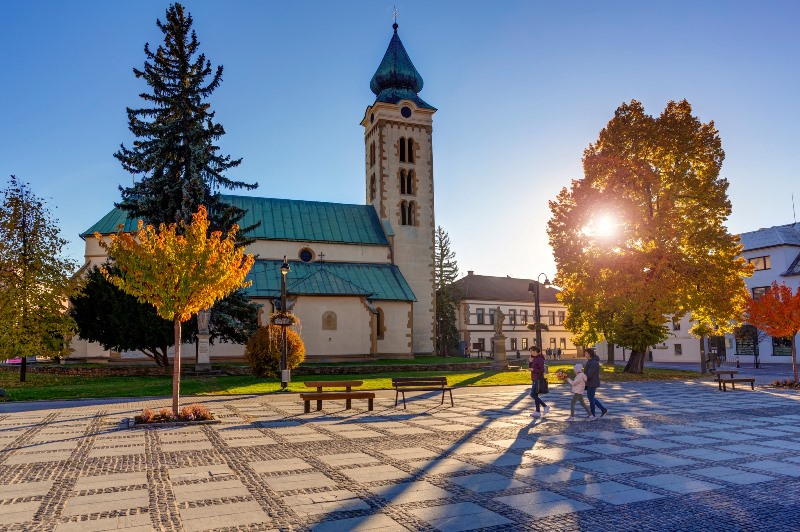
\includegraphics[width=\textwidth]{day4/mikulas}

		\pause
		\begin{itemize}
			\item Museum "Slovenské múzeum ochrany prírody a jaskyniarstva"
		\end{itemize}
	\end{frame}

	\section{Day 4. cost summarization}
	\begin{frame}
		\frametitle{Day 4. cost summarization}

		\begin{itemize}
			\item Bus ticket Mara -> Mikulas 11€
			\item Museum 5€
			\item CHALUPY TRI GROŠE VLAŠKY 20€
		\end{itemize}
	\end{frame}


	\section{Day 5.}

	\begin{frame}
		\frametitle{Rožňava}

		\only<1>{
			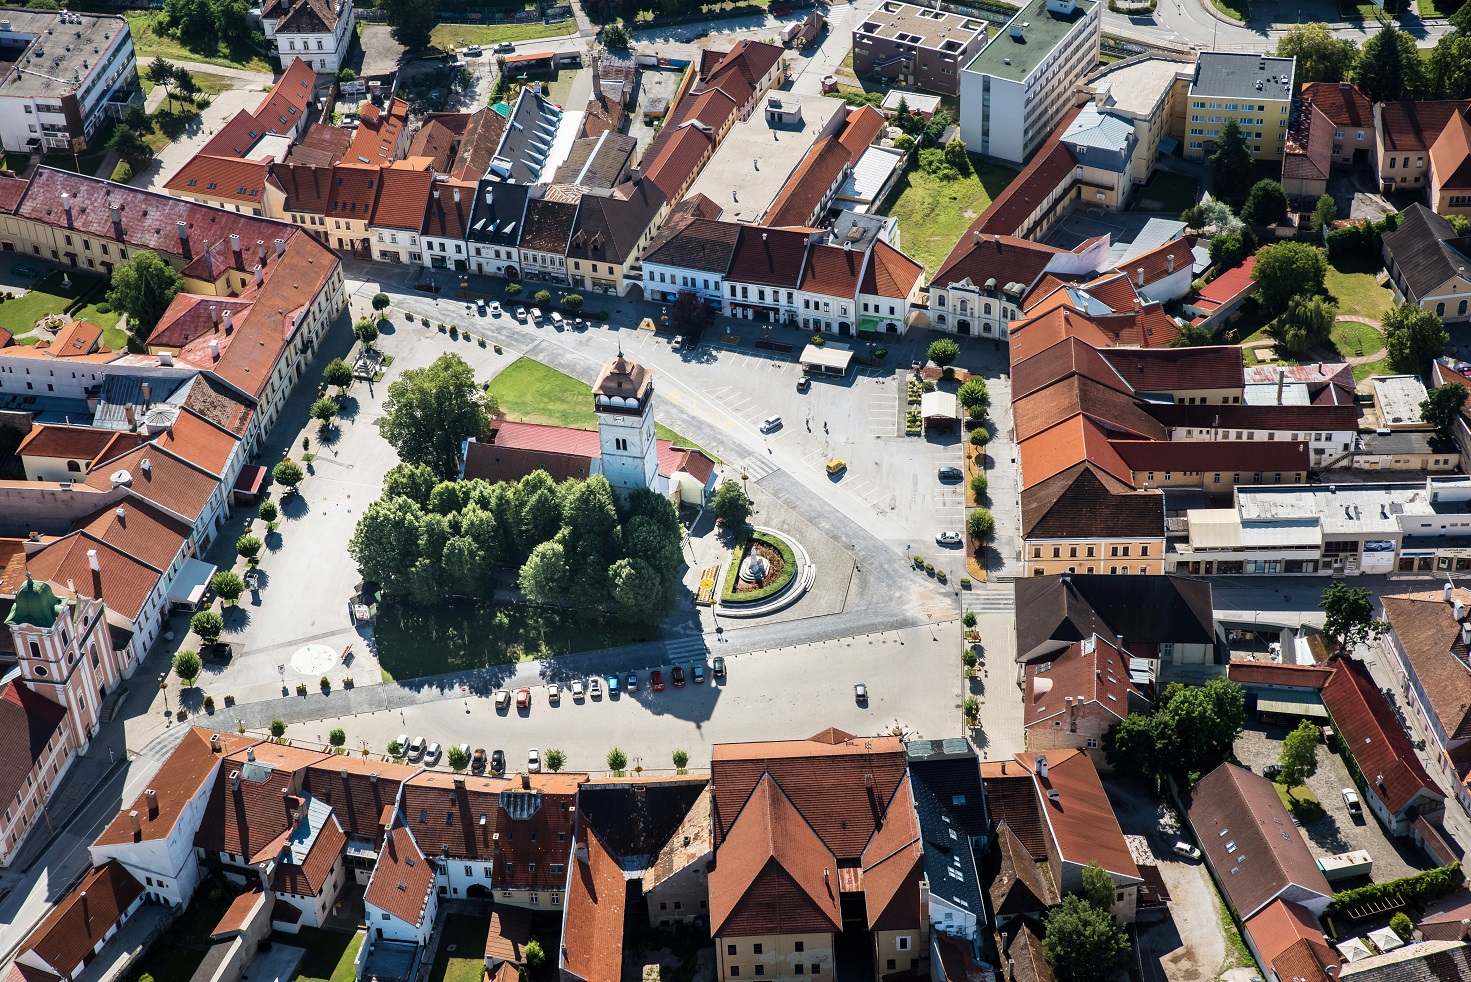
\includegraphics[width=\textwidth]{day5/roznava}
		}
		\only<2>{
			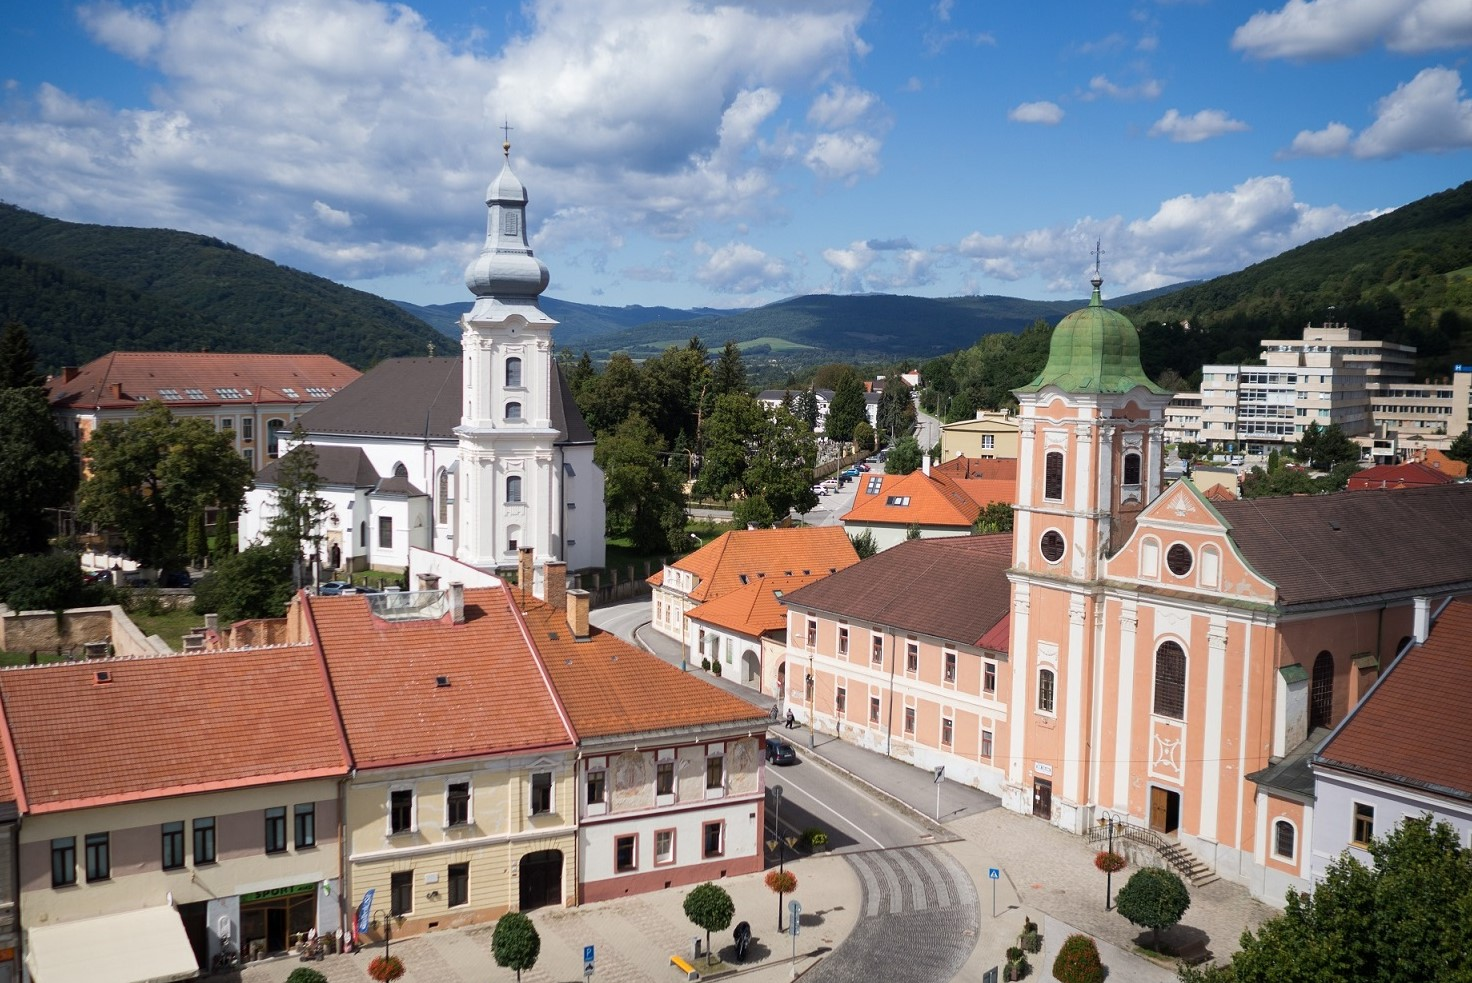
\includegraphics[width=\textwidth]{day5/roznava1}
		}
		\only<3>{
			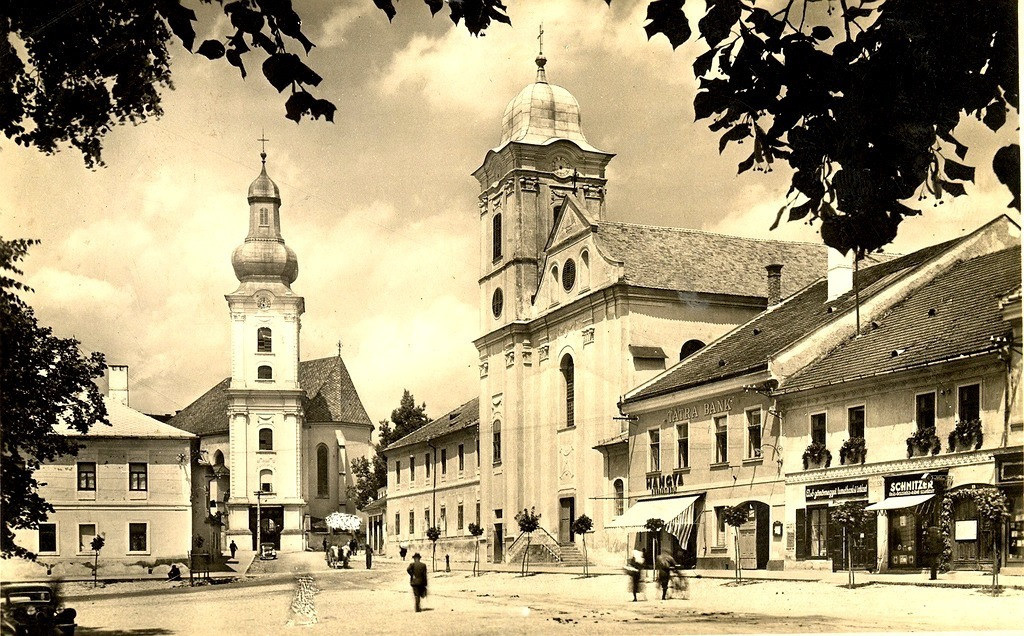
\includegraphics[width=\textwidth]{day5/roznava3}
		}
	\end{frame}

	\begin{frame}
		\frametitle{Back to the future}

		\only<1>{
			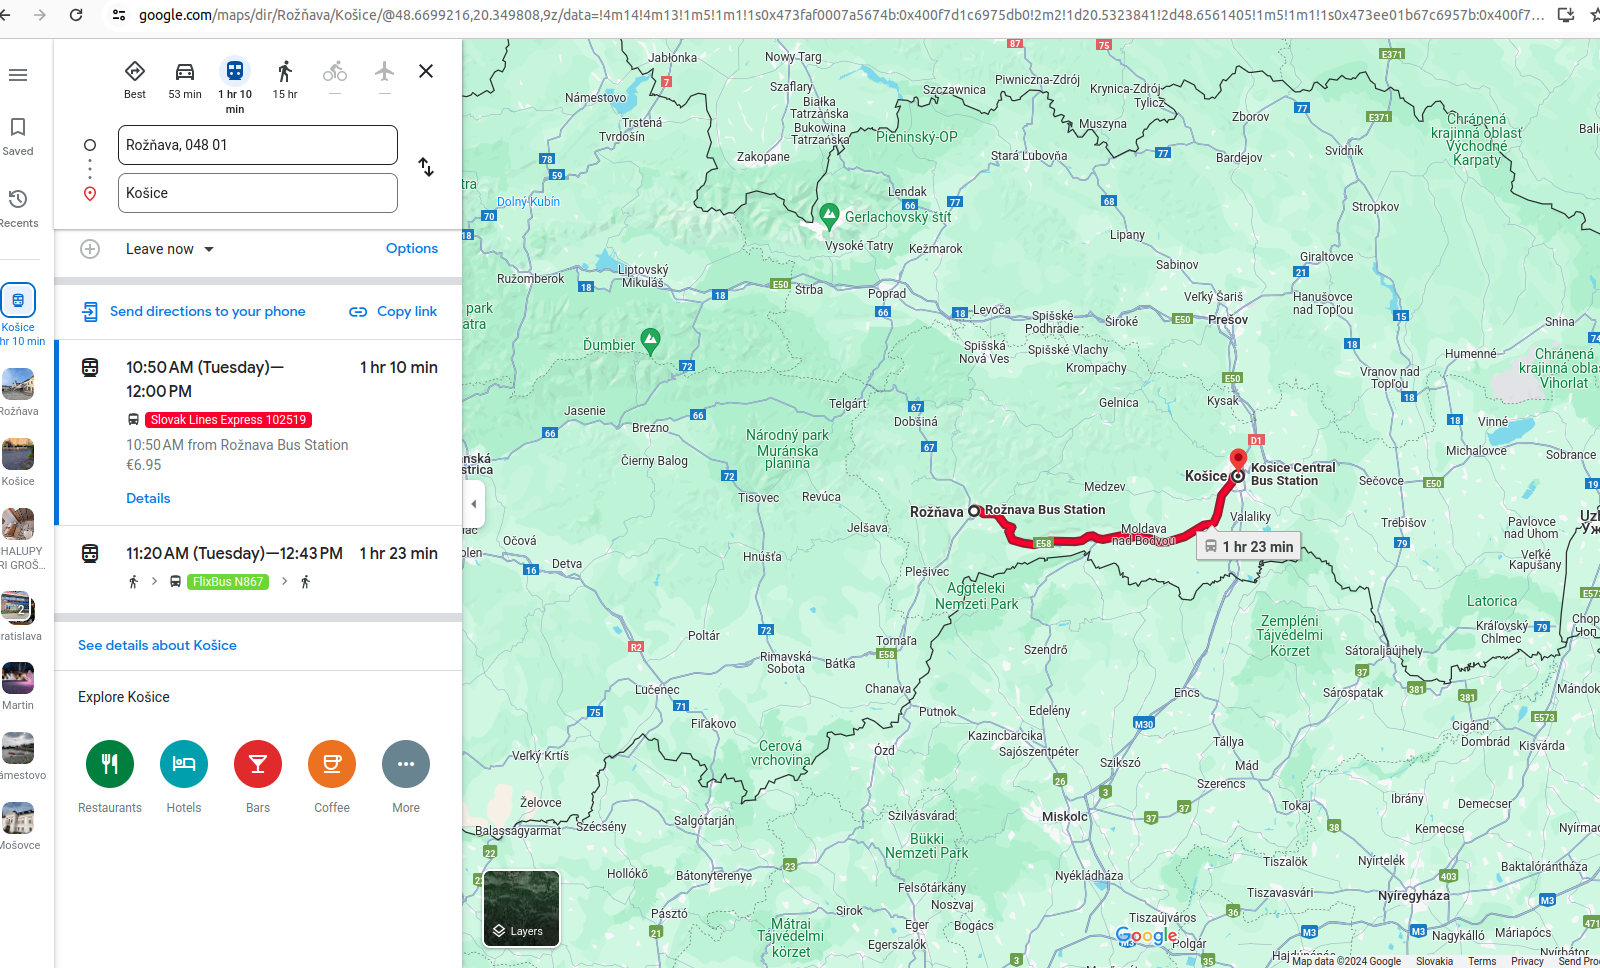
\includegraphics[width=\textwidth]{day5/bus}
		}
		\only<2>{
			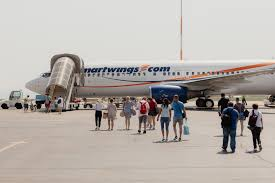
\includegraphics[width=\textwidth]{day5/boarding}
		}
	\end{frame}

	\section{Day 1-5 cost summary}

	\begin{frame}
		\frametitle{Day 5. cost summarization}

		\centering
		Grand total 172.8 euro\\[1em]
		
		\pause
		
\includegraphics[width=0.8\textwidth]{mission}
	\end{frame}	
	

	\begin{frame}
		\frametitle{Summarization}
		\begin{enumerate}
			\item Day 1
				\begin{itemize}
					\item Košice
				\end{itemize}
			\item Day 2.
				\begin{itemize}
					\item Spišský hrad
					\item Poprad
				\end{itemize}
			\item Day 3.
				\begin{itemize}
					\item High Tatras
					\item Veľké Hincovo pleso
					\item Štrba
					\item Poprad
				\end{itemize}
			\item Day 4.
				\begin{itemize}
					\item Liptovská Mara
					\item Liptovský Mikuláš
				\end{itemize}
			\item Day 5.
				\begin{itemize}
					\item Rožňava
					\item Košice
				\end{itemize}
		\end{enumerate}
	\end{frame}

\end{document}
